\chapter{量子测量与模型边界}

波函数、Wigner 函数和理想联合概率并不等于实验直接记录的量。实际数据通常是经过探测器响应、背景和计数噪声作用后的离散计数。能量分辨率会把相邻边带混在一起，OAM sorter 会串扰，探测效率会丢事件，背景还会把本来最敏感的低概率通道抬起来。若反演时把这些都放到最后再“修正”，很容易把仪器响应拟合成新的物理。

只有把理想散射概率、仪器响应和计数噪声写在同一个前向模型内，才能判断数据究竟识别了哪些参数。Fisher 信息与贝叶斯后验分别从局域灵敏度和完整概率分布回答这个问题；信号强度增加并不保证可辨识性同步改善。

实验数据用计数 $D_j$ 表示，模型预测的期望计数为 $\mu_j$；$R_{ji}$ 或 $K_{ji}$ 表示探测器响应矩阵，$b_j$ 为背景期望计数，$N$ 为信号计数尺度。参数向量记为 $\vb{\theta}$。Fisher 矩阵只描述给定似然模型下的局域可辨识性；当 $F$ 奇异或病态时，单纯增加总计数并不能消除参数退化。


\section{计数与估计}
参数估计必须从“实验实际记录什么”开始。设待估参数为向量 $\vb{\theta}$，理想物理模型在真实通道 $i$ 上给出归一化概率 $p_i(\vb{\theta})$。探测器的有限分辨率用响应矩阵 $R_{ji}=P(j\,|\,i)$ 表示。若 $j$ 包括未探测事件，或已条件化在成功探测的样本上，则 $\sum_jR_{ji}=1$；若只列出实际记录的通道且效率损失未并入 $N$，则允许 $\sum_jR_{ji}<1$。若总信号计数期望为 $N$，观测通道 $j$ 还有背景期望计数 $b_j$，则实际泊松均值是

\begin{equation}
\mu_j(\vb{\theta})=N\sum_iR_{ji}p_i(\vb{\theta})+b_j.
\label{eq:ch07-1}
\end{equation}

这里 $p_i$ 是无量纲概率，$\mu_j$ 是计数期望，二者不能混用。有限分辨率先通过 $R$ 把相邻真实通道混合，背景再增加与参数弱相关或无关的计数。只有把这两步写进前向模型，后面的误差条才对应真实实验。

若观测计数独立服从 $k_j\sim\operatorname{Pois}(\mu_j)$，对数似然为 $\log L=\sum_j[k_j\log\mu_j-\mu_j-\log(k_j!)]$。求导得分函数 $\partial_a\log L=\sum_j(k_j/\mu_j-1)\partial_a\mu_j$；利用 $\mathbb E(k_j)=\mu_j$ 和 $\operatorname{Var}(k_j)=\mu_j$，以及通道之间的独立性，得到 Fisher 信息矩阵

\begin{equation}
F_{ab}=\sum_j\frac{1}{\mu_j}\frac{\partial\mu_j}{\partial\theta_a}\frac{\partial\mu_j}{\partial\theta_b}.
\label{eq:ch07-2}
\end{equation}

式\cref{eq:ch07-2} 假定 $\mu_j>0$，或对零期望计数通道取适当极限。只有当参数改变了期望计数，且变化未被探测器模糊化，相关通道才提供非零信息。若探测器展宽把两个参数点映射成几乎相同的 $\mu_j$，相应导数就会变小，Fisher 信息随之下降。

对满足常规正则条件的局部无偏估计，协方差满足 Cramér--Rao 下界

\begin{equation}
\operatorname{Cov}(\hat{\vb{\theta}})\succeq F^{-1}.
\label{eq:ch07-3}
\end{equation}

只有当 $F$ 满秩时，$F^{-1}$ 才存在。若某个非零方向 $\mathbf u$ 满足 $F\mathbf u=0$，沿 $\mathbf u$ 改变参数在一阶上不会改变可测分布，数据就无法局部区分这一参数组合。这个秩条件比“信号够不够强”更基本。 例如，能量--OAM 的闭合交换历史只读取若干特定的相位差；即使有四路独立驱动，若实验只提供两条独立关系，测得的噪声衰减至多决定一个 $2\times2$ 的关系协方差，而无法确定四路相位噪声的全部十个协方差分量。具体的可运行逆问题见\cref{eq:oam-two-loop-gram,eq:oam-two-loop-fisher}。

当样本少、模型强非线性、参数受边界约束或似然多峰时，局部二次近似不够，应保留完整贝叶斯后验分布

\begin{equation}
p(\vb{\theta}|D)=\frac{p(D|\vb{\theta})p(\vb{\theta})}{\int \dd \vb{\theta}\,p(D|\vb{\theta})p(\vb{\theta})}.
\label{eq:ch07-4}
\end{equation}

因此 Fisher 信息回答局部可辨识性和渐近精度，贝叶斯后验回答有限数据下哪些参数区域仍然可信；二者都必须建立在同一个\cref{eq:ch07-1} 前向模型上。

\textsuperscript{\hyperref[ch07-ref4]{[4]}\hyperref[ch07-ref5]{[5]}}
任何反演都必须从探测器开始。理想边带、OAM 或联合通道经过有限分辨率以后，导数 $\partial q/\partial\theta$ 可能显著缩小；背景又会把原本低概率但高灵敏度的通道淹没。有限分辨率和背景首先改变实际计数分布；统计估计必须建立在这个已经卷积过的分布上。

\begin{figure}[!htbp]
\centering
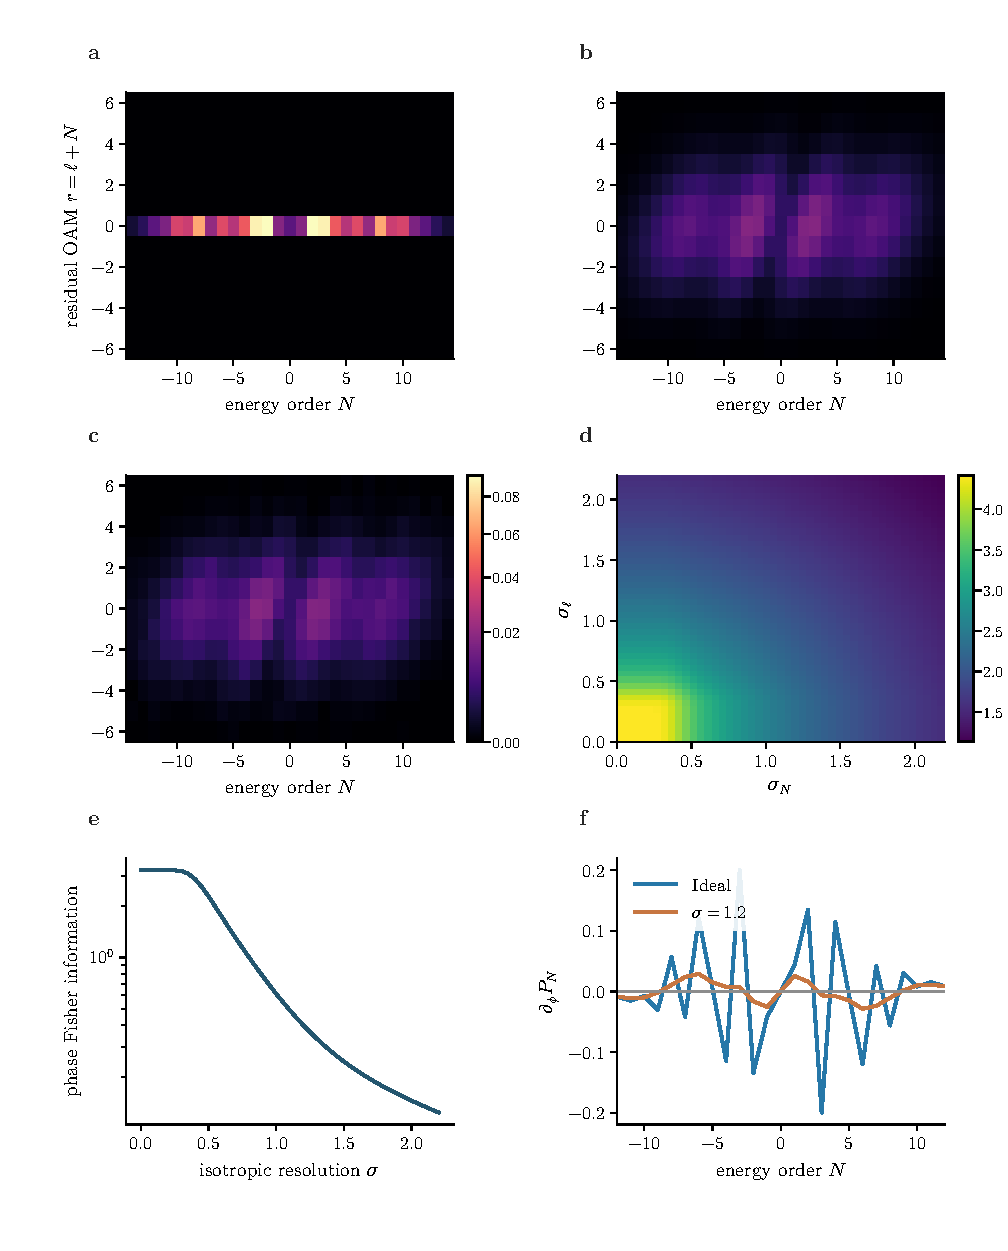
\includegraphics[width=0.96\linewidth,height=0.70\textheight,keepaspectratio]{observable_entanglement_metrology.pdf}
\caption{\textbf{有限分辨率下可观测的能量--OAM 信息}\quad 先从理想的能量--OAM 联合分布出发，再依次加入有限能量分辨率、有限 OAM 分辨率和泊松计数噪声。探测器把原本清晰的联合结构卷积并稀释，因此可测互信息和相位 Fisher 信息都会下降。 最后比较理想与有限分辨率下能量边际人口对相位的导数，从而看出敏感信息在谱线上怎样分布。前三幅热图改用剪切坐标 $r=\ell+N$：理想选择定则为 $r=0$，探测器造成的展宽沿 $r$ 方向直观可见；三个图使用相同概率色标，绘制范围包含超过 $99\%$ 的概率。}
\label{fig:ch07-novel-extensions--05-observable-entanglement-metrology}
\end{figure}

数值实现中，探测器卷积及独立泊松计数的前向模型为
\[\begin{aligned}
q_{ij}&=\sum_{N,L}K_{ij|NL}(\sigma_N,\sigma_L)P_{NL},&\quad Y_{ij}&\sim\operatorname{Poisson}(N_eq_{ij}),\\
I(N{:}L)&=\sum_{NL}q_{NL}\log_2\frac{q_{NL}}{q_Nq_L},& F_{\phi\phi}&=\sum_{ij}\frac{(\partial_\phi q_{ij})^2}{q_{ij}}.
\end{aligned}\]
本图选取退化映射 $|\beta_1|=|\beta_2|=2$、$\ell_1=-1$、$\ell_2=-2$，使 $\det A=\ell_2-2\ell_1=0$：不同两色路径落到同一 $(N,L)$，于是能够发生相位敏感的振幅干涉；这并不是合成维度章节用于展开二维格点的可逆配置。相位基准取 $\theta_1=0,\theta_2=-\pi/2$，有限差分步长 $\delta\theta_2=10^{-3}$。在无额外模式混合、且 $\det A\ne0$ 的理想可逆方案里，每个输出点只有一条路径，\emph{纯人口测量}对 $\theta_2$ 的 Fisher 信息反而为零。有限分辨率示例 $\sigma_N=\sigma_L=1.2$（以边带阶数计），泊松数据 $N_e=25000$、随机种子 2。分辨率图每轴 $[0,2.2]$（45 点），模拟高斯模糊采用 $\texttt{scipy.ndimage.gaussian\_filter}$ 的零边界延拓再整体归一化；(c) 的原始计数为各像素独立 Poisson 抽样后除以观测总数。Fisher 剖面使用截断 $n_{\max}=10$，参考测量 $\sigma_N=\sigma_L=0.8$；数值 Fisher 求和分母截断为 $\max(q_{ij},10^{-14})$，(e) 对数图显示地板为 $10^{-8}$。(f) 对相同相位点以 $\delta\phi=10^{-3}$ 做中心差分，比较理想与 $\sigma_N=\sigma_L=1.2$ 时的 $\partial_\phi P_N$；所有能量边际均从二维前向概率逐 OAM 求和。


Fisher 信息适合回答“在某个已知参数附近，小扰动能被多精确地区分”，贝叶斯后验分布则回答“给定实际有限数据，哪些参数值仍然可信”。当后验分布单峰且样本足够大时，两者应相互一致；若不一致，往往意味着非线性、多峰或边界效应已经重要。


在电子显微实验里，弱信号最常见的困难并不是公式上没有响应，而是响应小到被背景、探测器噪声或漂移淹没。自由电子 Ramsey 成像已经实验证明，第二次相干参考作用可以把弱近场调制转成强干涉信号，并在 2024 年实现约二十倍的相干信号放大。\textsuperscript{\hyperref[ch07-ref6]{[6]}} 但这类相干放大并不自动意味着突破散粒噪声极限：理想无背景条件下，局域振荡器可以把信号搬到更容易检测的通道，却不会凭空增加样品对未知参数携带的量子 Fisher 信息。

更高阶的能量--OAM 观测也有同样的问题：单纯改变读出端口的随机混合不能增加信息，但在样品场上叠加已知相干参考，会改变相互作用的散射振幅。\cref{fig:oam-reference-rescue} 比较了参考辅助的一光子读出与无参考的高阶 OAM 读出，并将没有进入目标边带的电子纳入统计；这种改变实验设置的增益不违背下面的信息处理不等式。

这一区分可以直接写进前向模型。设样品弱耦合为 $g(\theta)$，参考耦合为已知的 $g_r \ee^{\ii\phi_r}$。在弱样品极限，干涉项使期望计数出现对 $g$ 的线性响应，
\begin{equation}
\mu(\phi_r;\theta)\simeq \mu_0+2A|g_r|\operatorname{Re}\!\left[g(\theta)\ee^{-\ii\phi_r}\right],
\label{eq:ch07-homodyne-forward}
\end{equation}
而没有参考时常见信号从 $|g|^2$ 起步。若实验受固定读出噪声或背景限制，线性化会显著提高实际可见度；若只受理想泊松散粒噪声限制，则必须用\cref{eq:ch07-2} 重新计算 Fisher 信息，不能把“峰变高了”直接写成“灵敏度提高同样倍数”。

2026 年 Velasco 与 García de Abajo 提出的自由电子量子计量方案讨论的是更强的一层：让电子沿波导以长有效作用长度发生强相位匹配耦合，使单电子能够交换数十个导模光子，再把电子束分器、两次电子--波导作用和电子电流读出组合起来。论文理论上预测可用当前可达参数把光学相位灵敏度提高约一个数量级，并讨论高光子数 NOON 态的电子后选择制备。\textsuperscript{\hyperref[ch07-ref7]{[7]}} 这里的资源不只是“参考场更强”，而是强电子--光子耦合加上电子路径叠加共同改变了可访问的量子态和测量算符。

因此本章后面的最优设计要分两步。第一步问给定实验架构的 Fisher 信息怎样随耦合、参考相位、波长和剂量变化；第二步才问是否存在另一个量子态或测量基，使可达到的 Fisher 信息上界本身提高。把这两步混在一起，会把工程信噪比改进误写成量子增强，也会把真正的量子资源埋在“更多计数”里。

\textsuperscript{\hyperref[ch07-ref8]{[8]}}
高能 PINEM 常同时占据许多能量阶，因此最自然的语言是量子行走和贝塞尔边带。2026 年 10 月 Pan、Zhang 与 Podolsky 讨论了相反的低能 Bragg 区：利用反冲把非共振能量通道分开，只保留两个近共振合成能量态，于是自由电子可以像一个真正的二能级系统那样做 $\pi/2$ 和 $\pi$ Rabi 操作，并把这些操作用作近场量子干涉仪的分束器与反射镜。

一旦只保留两个近共振态 $|g\rangle,|e\rangle$，最小有效哈密顿量就是
\begin{equation}
H_{2}=\frac{\hbar}{2}
\begin{pmatrix}
-\Delta & \Omega \ee^{-\ii\phi}\\
\Omega \ee^{\ii\phi} & \Delta
\end{pmatrix},
\label{eq:ch07-twolevel-electron}
\end{equation}
其中 $\Omega$ 是由近场决定的有效 Rabi 频率，$\Delta$ 是两能级失谐，$\phi$ 保留近场相位。若初态为 $|g\rangle$，作用时间为 $\tau$，激发概率为
\begin{equation}
P_e(\tau)=\frac{\Omega^2}{\Omega^2+\Delta^2}
\sin^2\!\left(\frac{\tau}{2}\sqrt{\Omega^2+\Delta^2}\right).
\label{eq:ch07-rabi-probability}
\end{equation}
在共振处，$\Omega\tau=\pi/2$ 产生等权叠加，可充当能量空间分束器；$\Omega\tau=\pi$ 交换两态，可充当镜面。把两个 $\pi/2$ 操作夹在未知近场作用前后，就得到能量空间 Ramsey/Mach--Zehnder 型干涉仪，输出人口直接依赖未知场的幅度和相位。

这个构造对“测量”一章尤其重要，因为它把连续多边带拟合变成了接近标准量子传感的二能级读出。若未知近场主要造成小相位 $\varphi$，理想二端口概率可写成
\begin{equation}
p_\pm(\varphi)=\frac{1\pm\mathcal V\cos(\varphi+\varphi_0)}{2},
\label{eq:ch07-twolevel-fringes}
\end{equation}
于是单电子对 $\varphi$ 的经典 Fisher 信息为
\begin{equation}
F_1(\varphi)=\sum_{s=\pm}\frac{[\partial_\varphi p_s]^2}{p_s}.
\label{eq:ch07-twolevel-fisher}
\end{equation}
令 $\Phi=\varphi+\varphi_0$，代入两端口概率可算得 $F_1=\mathcal V^2\sin^2\Phi/(1-\mathcal V^2\cos^2\Phi)$。当 $\mathcal V=1$ 且两端口概率均非零时，$F_1=1$；有限对比度、泄漏到第三个能量阶以及探测器串扰都会把它压低。这样就能把“二能级电子看起来更干净”变成可比较的单位剂量信息量，而不是只比较条纹视觉对比度。

论文还指出，若近场本身量子化，二能级电子可以出现量子和真空 Rabi 振荡，从而探测光场量子统计与电子--光子纠缠。这里必须保持证据等级：截至本书截稿日，这一工作提出的是理论量子谱学方案；它的重要性在于给出了从低能反冲、合成能量二能级到量子近场读出的闭合模型，而不是已经完成了真空 Rabi 的实验观测。


\textsuperscript{\hyperref[ch07-ref9]{[9]}}
前面的测量问题主要把未知参数放在经典近场、几何或光子统计里。Crispin 与 Talebi 2026 年的工作把目标换成一个任意初态的量子发射体，并问自由电子能否直接读取其量子相干性。其关键预测是：若发射体初态包含能级间相干项，电子不仅看到普通能损通道，零损失峰概率本身也会随相干演化出现振荡，并对发射体跃迁频率敏感。

这个现象可以用最小干涉模型理解。设二能级发射体初态密度矩阵为
\begin{equation}
\rho_a=
\begin{pmatrix}
\rho_{gg}&\rho_{ge}\\
\rho_{eg}&\rho_{ee}
\end{pmatrix},
\label{eq:ch07-emitter-rho}
\end{equation}
电子某个输出能量通道 $m$ 的概率一般具有
\begin{equation}
P_m=\rho_{gg}P_m^{(g)}+\rho_{ee}P_m^{(e)}
+2\operatorname{Re}\!\left[\rho_{ge}\,A_m^{(g)}A_m^{(e)*}\right].
\label{eq:ch07-coherence-interference}
\end{equation}
前两项只依赖人口，第三项才直接依赖量子相干。若电子与发射体的两条散射路径在最终测量中不可区分，$\rho_{ge}$ 就能以干涉项进入电子谱；若环境或探测器把两条路径完全区分，第三项会被抹掉。因此“电子谱是否看见相干性”本质上仍是一个哪一路信息问题。

如果自由演化使 $\rho_{ge}(t)=\rho_{ge}(0)\ee^{-\ii\omega_0t-\Gamma_2t}$，那么扫描电子到达延迟 $t$ 时，某些电子谱通道会出现频率 $\omega_0$ 的振荡包络。Crispin--Talebi 的完整量子理论指出零损失峰就是一个清楚的相干指纹。实验设计上，这比单纯追求更大的能损概率更微妙：最优通道应最大化对 $\operatorname{Re}\rho_{ge}$、$\operatorname{Im}\rho_{ge}$ 或 $\omega_0$ 的 Fisher 信息，而不一定是计数最多的边带。

这也给“量子态层析”提供了另一条路线。若改变电子入射相位、到达时间或预整形态能够旋转 $A_m^{(g)}A_m^{(e)*}$ 的复相位，就可以分别读取 $\rho_{ge}$ 的两个正交分量。于是实验设计从“用电子测一个谱”升级为“用一组受控电子探针实现发射体 POVM”。真正需要验证的不是是否出现振荡，而是不同人口/相干模型在完整探测器前向模型下是否可辨识。


局部统计精度再好，也不能解决前向映射本身不唯一的问题。因此在讨论测量资源如何分配之前，还要明确什么时候复耦合场的幅度和相位可以被分开恢复。
若未知量是复耦合 $\beta(\vb{R})$，只测单个边带人口通常主要约束 $|\beta|$，而不能唯一恢复 $\arg\beta$。要得到相位，需要加入已知参考耦合或改变测量基，使观测概率含有 $\beta$ 与参考场的干涉项。四相位参考测量就是把复数的两个正交分量转成可测人口差。

多参数几何反演也有同样问题。定义灵敏度矩阵 $J_{ja}=\partial\mu_j/\partial\theta_a$ 和权重矩阵 $W=\operatorname{diag}(1/\mu_j)$，则

\begin{equation}
F=J^{\mathsf T}WJ.
\label{eq:ch07-5}
\end{equation}

若 $J$ 的两列几乎平行，两个参数改变数据的方式几乎相同，$F$ 就会出现很小的本征值；误差椭圆沿该本征向量被拉长。加入另一波长、偏振或参考相位的目的不是简单增加数据量，而是让新的灵敏度方向与原方向不平行，从而抬高最小本征值并打破退化。

\begin{figure}[!htbp]
\centering
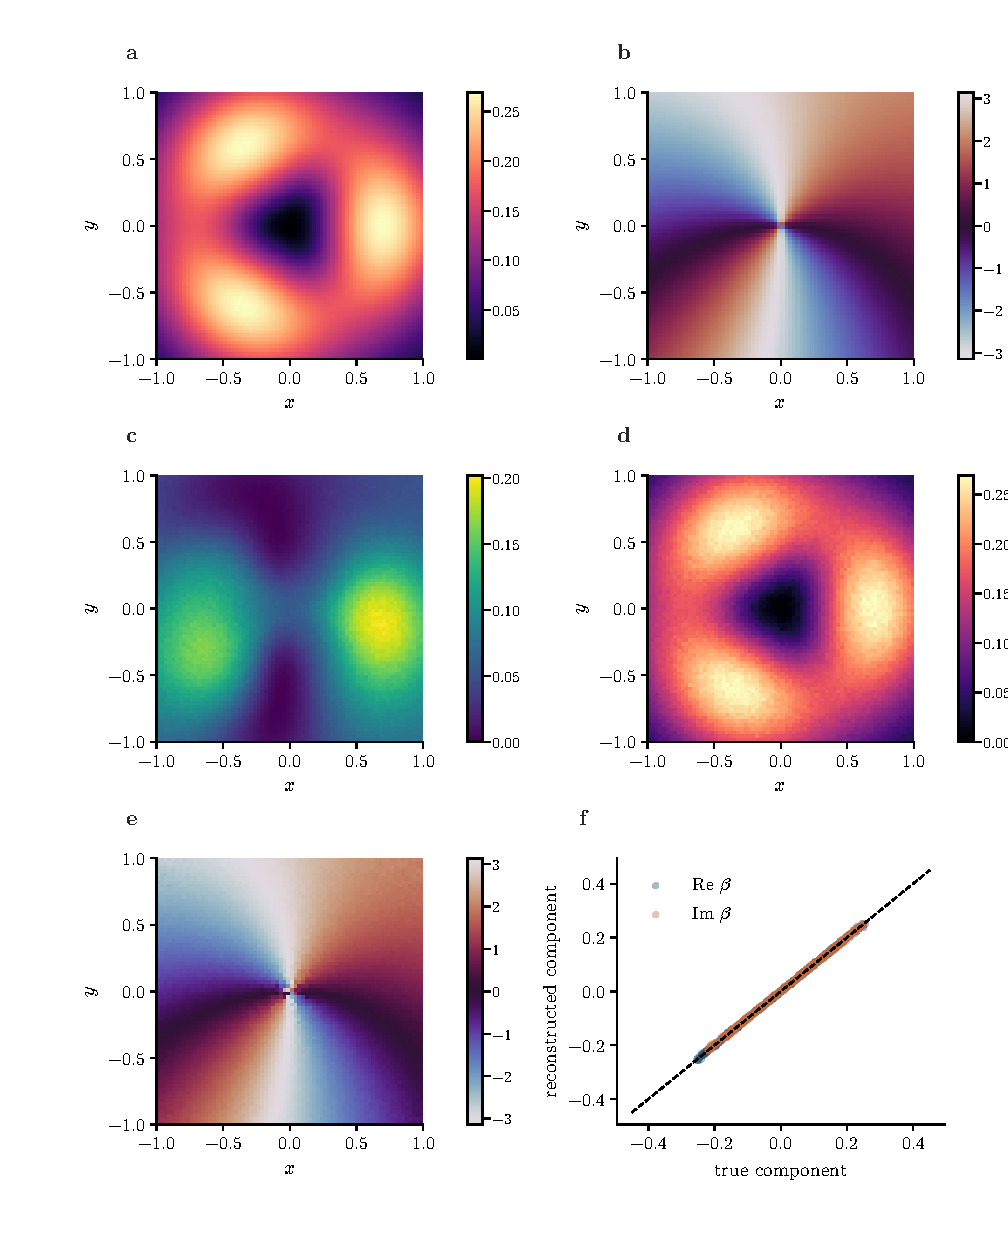
\includegraphics[width=0.96\linewidth,height=0.70\textheight,keepaspectratio]{complex_beta_field_tomography.pdf}
\caption{\textbf{参考场怎样恢复复耦合的振幅和相位}\quad 只测单次 PINEM 边带人口时，概率主要由 $|\beta|$ 决定，因此相位信息不能唯一恢复。加入已知参考耦合 $\beta_{\mathrm{ref}}\ee^{\ii\phi_r}$ 后，测得的边带概率依赖 $|\beta+\beta_{\mathrm{ref}}\ee^{\ii\phi_r}|$，改变参考相位就把复数的两个正交分量转成可测的人口变化。 用多组参考相位联合拟合，可以同时恢复 $\operatorname{Re}\beta$ 和 $\operatorname{Im}\beta$。重构是否稳定仍取决于参考场幅度、计数和探测分辨率；参考场过弱时，相位方向的 Fisher 信息会迅速下降。}
\label{fig:ch07-novel-extensions--29-complex-beta-field-tomography}
\end{figure}

数值实现中，复近场的干涉前向模型与四步相移反演采用
\[\beta(x,y)=1.2(x^2+y^2)e^{-2(x^2+y^2)}\bigl[1+0.22\cos(3\operatorname{atan2}(y,x))\bigr]\ee^{\ii\Phi(x,y)},\quad \Phi=2\operatorname{atan2}(y,x)+0.8x-0.35y,\]
\[\beta_r=\beta+0.25\ee^{\ii\phi_r},\quad \phi_r\in\{0,\tfrac\pi2,\pi,\tfrac{3\pi}2\},\quad q_r=J_1^2(2|\beta_r|),\quad Y_r\sim\operatorname{Poisson}(N_eq_r).\]
反演先在单调的第一贝塞尔支上数值反求有效强度 $R_r=|\beta_r|^2$：使用 $r\in[0,2.2]$ 的 2400 点查找表，并只保留 $J_1^2(2r)$ 第一个极大值以前的支段；随后执行
\[\operatorname{Re}\widehat\beta=\frac{R_0-R_\pi}{4(0.25)},\qquad \operatorname{Im}\widehat\beta=\frac{R_{\pi/2}-R_{3\pi/2}}{4(0.25)}.\]
这里采用绕数为整数 $m=2$ 的连续涡旋场；振幅包含 $r^2$ 因子，使相位不定的原点同时成为振幅零点，避免在非零场处人为引入角向支割。空间网格 $x,y\in[-1,1]$，各 72 点；泊松总计数参数 $N_e=30000$，随机种子 9。相对均方重建误差只在真值 $|\beta|>0.08$ 上统计；(f) 的散点比较在 $|\beta|>0.06$ 上按序每 8 点抽样。这里是经贝塞尔标定的四步相移算法，\emph{不是}通用加权非线性最小二乘求解；主要误差来自泊松计数与第一支查表近似。


\medskip
\section{相位与 Fisher 信息}
\noindent 仅仅知道复耦合的模长，还不能回答纳米近场的相位是什么。前面的四步参考成像利用第一条边带的贝塞尔曲线反推出模长，但当 $J_1^2$ 越过第一个极大值，同一个边带概率可能对应多个不同耦合强度，必须额外选择分支。我们可以改测\emph{整个能量谱的二阶矩}：它虽然需要收集多个边带，却有一个不依赖弱耦合近似的恒等式，因而不需要反演贝塞尔函数的单调支。

设样品和参考光作用于同一电子的\emph{相同光学频率}，两段作用之间的自由传播不足以改变边带之间的相干相位；两个能量平移生成元相互对易。已知参考复耦合为 $B\ee^{\ii\phi_r}$，其中 $B>0$ 已校准，样品未知耦合写作 $\beta=x+\ii y$。于是总相位调制算符的指数直接相加，有
\begin{equation}
\beta_{\mathrm{tot}}(\phi_r)=x+\ii y+B\ee^{\ii\phi_r},\qquad
P_n(\phi_r)=J_n^2\!\left(2|\beta_{\mathrm{tot}}(\phi_r)|\right).
\label{eq:phase-reference-composition}
\end{equation}
这里 $x$ 和 $y$ 是相对于参考相位零点定义的无量纲笛卡尔分量，并不是两个独立的光强。倘若两次作用频率不同、电子在中间发生可观的色散，或者光学相位在扫描期间漂移，就必须重新使用相应的传播算符和退相干模型，而不能把两次相互作用简单相加。

为什么二阶谱矩比单条边带更容易处理？令 $g=|\beta_{\mathrm{tot}}|$，相位波函数 $f(\vartheta)=\exp[2\ii g\sin\vartheta]$ 的 Fourier 系数就是 $J_n(2g)$。利用 Fourier 系数的正交性，把特征函数写成同一波函数与其平移副本的重叠，逐步得到
\begin{align*}
\Phi(t)&\equiv\sum_{n=-\infty}^{\infty}P_n\ee^{\ii nt}
=\frac{1}{2\pi}\int_{-\pi}^{\pi}\dd\vartheta\,f(\vartheta+t)f^*(\vartheta)\\
&=\frac{1}{2\pi}\int_{-\pi}^{\pi}\dd\vartheta\,
\exp\!\left[2\ii g\bigl(\sin(\vartheta+t)-\sin\vartheta\bigr)\right]\\
&=\frac{1}{2\pi}\int_{-\pi}^{\pi}\dd u\,
\exp\!\left[4\ii g\sin(t/2)\cos u\right]
=J_0\!\left(4g\sin\frac{t}{2}\right).
\end{align*}
第二行使用了三角恒等式，并在积分变量中平移 $u=\vartheta+t/2$；周期性保证积分区间平移不改变结果。将 $\sin(t/2)=t/2-t^3/48+O(t^5)$ 和 $J_0(z)=1-z^2/4+z^4/64+O(z^6)$ 代入，得到
\[
\Phi(t)=1-g^2t^2+\left(\frac{g^2}{12}+\frac{g^4}{4}\right)t^4+O(t^6).
\]
对特征函数在原点求导，于是\emph{未经截断的}理想 PINEM 能谱满足
\begin{equation}
\langle n^2\rangle=2g^2,\qquad
\langle n^4\rangle=2g^2+6g^4.
\label{eq:phase-reference-moments}
\end{equation}
这两式直接连接多条边带，不依赖相互作用有多弱。若能量增益和损失通道都被准确收集，用整张能谱的二阶矩就能读取 $g^2$。如果仅记录有限个通道，或探测器对大阶数有不同效率，则须先在前向模型中处理截断和效率，不能直接把测得的截断矩当成全谱矩。

把参考场写入 $g^2=|\beta+B\ee^{\ii\phi_r}|^2$，二阶矩的四相位结构立即成为
\begin{equation}
Y(\phi_r)\equiv\frac{\langle n^2\rangle_{\phi_r}}{2}
=x^2+y^2+B^2+2B(x\cos\phi_r+y\sin\phi_r).
\label{eq:phase-reference-second-moment}
\end{equation}
将参考相位依次取为 $0,\pi/2,\pi,3\pi/2$，相对的两组相位差分分别只保留 $x$ 与 $y$：
\begin{equation}
\widehat x=\frac{\widehat Y(0)-\widehat Y(\pi)}{4B},\qquad
\widehat y=\frac{\widehat Y(\pi/2)-\widehat Y(3\pi/2)}{4B}.
\label{eq:phase-reference-quadratures}
\end{equation}
这是一种精确的代数解调关系，并不需要先假设 $|\beta|\ll1$；但它需要非零的、相位稳定且幅值已知的参考场。光学相位只相对参考才有意义，若参考零点本身未知，反演的 $(x,y)$ 也将整体旋转一个未知角度。

实验能量读数还包含入射能量散布与探测器展宽。令扣除平均能量后的无量纲读数 $u=(E-E_0)/(\hbar\omega)=n+\zeta$，把所有独立且不随参考相位变化的高斯展宽合并为 $\zeta\sim\mathcal N(0,s^2)$。由于 $\langle n\rangle=\langle\zeta\rangle=0$ 且二者独立，
\begin{equation}
\frac{\langle u^2\rangle_{\phi_r}}{2}
=Y(\phi_r)+\frac{s^2}{2}.
\label{eq:phase-reference-blurred-moment}
\end{equation}
四相位差分会消去相同的 $s^2/2$，所以\cref{eq:phase-reference-quadratures} 对这种\emph{共同、稳定}的高斯展宽仍然成立；这并不意味着分辨率无关紧要，因为展宽必然增加估计方差。

为了把这种增加精确算出来，先展开四次幂，再利用独立性和高斯四阶矩 $\langle\zeta^4\rangle=3s^4$：
\begin{align*}
\langle u^4\rangle
&=\langle n^4\rangle+6\langle n^2\rangle s^2+3s^4\\
&=2g^2+6g^4+12g^2s^2+3s^4.
\end{align*}
若每个参考相位测量 $M$ 个独立电子，用样本均值
$\widehat Y_r=M^{-1}\sum_{k=1}^M u_{r,k}^2/2$，可以不经渐近近似地得到
\begin{equation}
\operatorname{Var}(\widehat Y_r)=
\frac{g_r^2+g_r^4+4g_r^2s^2+s^4}{2M},\qquad
 g_r=|\beta+B\ee^{\ii\phi_r}|.
\label{eq:phase-reference-moment-variance}
\end{equation}
四组记录互相独立时，\cref{eq:phase-reference-quadratures} 给出
\[
\operatorname{Var}(\widehat x)=\frac{\operatorname{Var}(\widehat Y_0)+\operatorname{Var}(\widehat Y_{\pi})}{16B^2},\quad
\operatorname{Var}(\widehat y)=\frac{\operatorname{Var}(\widehat Y_{\pi/2})+\operatorname{Var}(\widehat Y_{3\pi/2})}{16B^2}.
\]
这些公式使“参考场能放大相位信息”的说法变得可检查：当 $B$ 太小时，差分信号被 $1/B$ 放大；当 $B$ 变大时，谱矩自身的统计涨落也增长。最优参考场因此依赖测量目标、剂量和探测响应，不能只把参考强度一直增大。

\begin{figure}[!htbp]
\centering
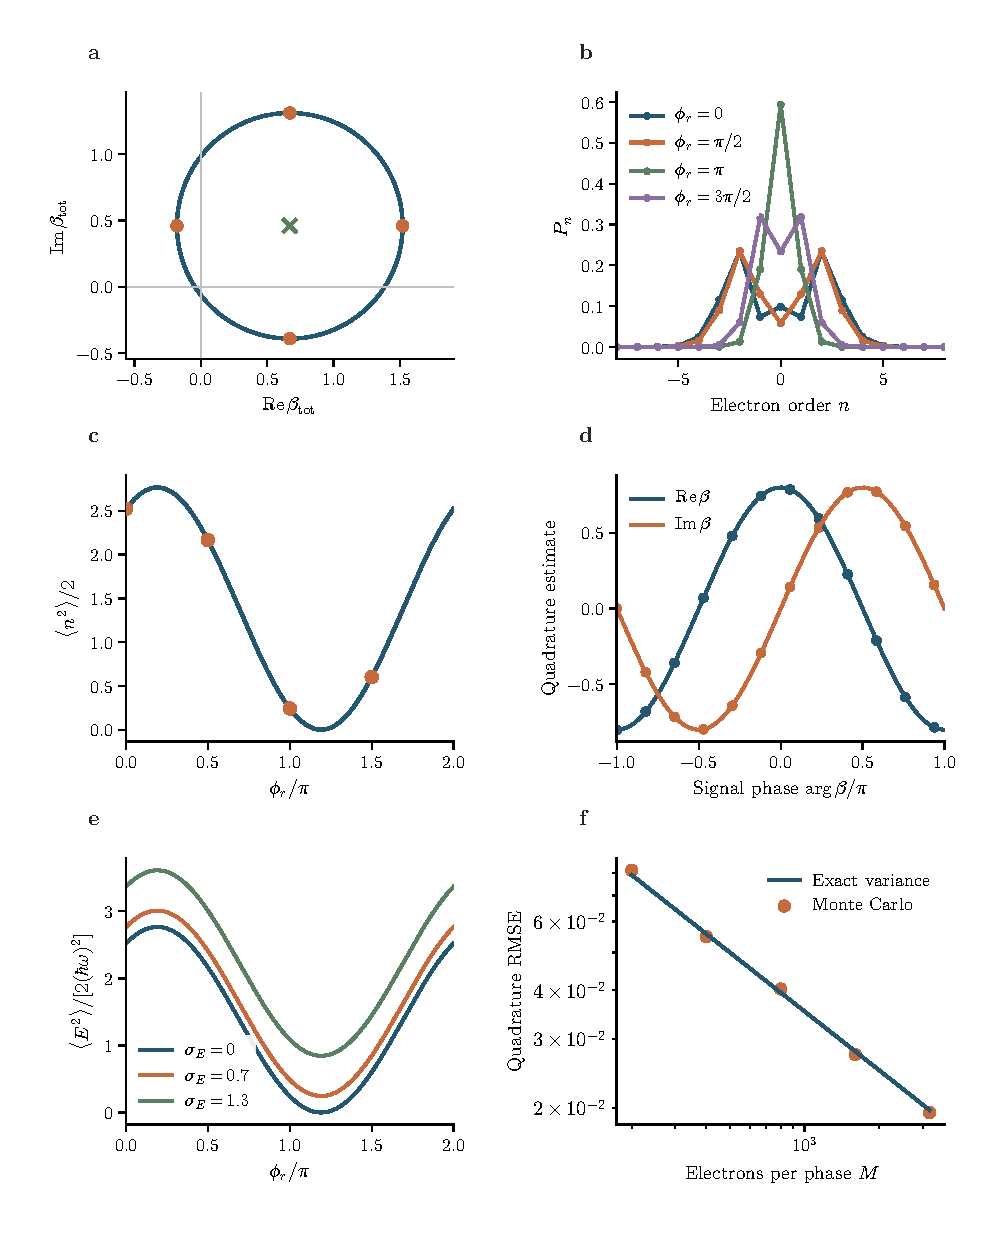
\includegraphics[width=0.96\linewidth,height=0.70\textheight,keepaspectratio]{phase_reference_response.pdf}
\caption{\textbf{四相位参考的复耦合与谱矩反演。} (a) 样品复耦合为固定点，扫描参考相位后总耦合在复平面上沿圆周移动；(b) 四个参考相位的完整贝塞尔边带分布；(c) 二阶谱矩随参考相位的精确正弦响应以及四个实际采样相位；(d) 改变样品相位时从四次二阶矩差分重构 $\operatorname{Re}\beta$、$\operatorname{Im}\beta$；(e) 相同高斯能量模糊只增加二阶矩的共同偏置；(f) 有限电子数下的复耦合重构均方根误差，解析方差与蒙特卡洛抽样相符合。图中没有将离散边带强行近似为连续高斯能谱。}
\label{fig:phase-reference-response}
\end{figure}

数值实现中，将样品复耦合写为 $\beta=x+\ii y$，真值设为 $x=0.67$、$y=0.46$，已校准的同频参考幅值 $B=0.85$。四个相位依次为 $\phi_r\in\{0,\pi/2,\pi,3\pi/2\}$，所有理想能谱由 $P_n=J_n^2(2|\beta+B\ee^{\ii\phi_r}|)$ 直接给出，数值保留 $n=-15,\ldots,15$。(a) 令 $\phi_r$ 在 $[0,2\pi]$ 上取 340 点绘 $\beta_{\mathrm{tot}}$ 复平面圆轨迹；(b) 画四个 $P_n$ 分布并显示 $-8\le n\le8$；(c) 按 $Y(\phi_r)=|\beta+B\ee^{\ii\phi_r}|^2$ 画谱矩曲线及四相位点；(d) 令 $\beta=0.8\ee^{\ii\varphi}$，$\varphi\in[-\pi,\pi]$ 取 160 点，按\cref{eq:phase-reference-quadratures} 计算恢复值并与真值对照；(e) 分别取总高斯展宽 $s=0,0.7,1.3$（以 $\hbar\omega$ 为单位），展示 $\langle u^2\rangle/2=Y+s^2/2$；(f) 固定 $s=0.7$，每相位计数 $M=200,400,800,1600,3200$，每个计数进行 180 次独立模拟，从 $n$ 的离散贝塞尔分布取样后加独立高斯误差 $\zeta$，以固定种子 $20261009+M$ 生成；橙色散点为 $\sqrt{\mathbb E[(\hat x-x)^2+(\hat y-y)^2]}$ 的模拟值，蓝线由\cref{eq:phase-reference-moment-variance} 的独立样本方差给出。模拟的有限 $n$ 截断在这些耦合强度下对归一化无可见影响。


二阶矩反演易于解释，却不一定是对全部事件信息最有效的估计。若记录每个电子的能量，具有宽度 $s$ 的高斯响应先把离散边带映射为连续能量分布 $q(u)$；实际像素 $j$ 上的概率应写成
\begin{equation}
q_j(\vb\theta,\phi_r)=\sum_n R_{jn}(s)
J_n^2\!\left(2|\beta+B\ee^{\ii\phi_r}|\right),\qquad
R_{jn}=\int_{u_j^-}^{u_j^+}\frac{\dd u}{\sqrt{2\pi}s}
\exp\!\left[-\frac{(u-n)^2}{2s^2}\right],
\label{eq:phase-reference-response-kernel}
\end{equation}
其中 $\vb\theta=(x,y)$。对四个相位采用相同剂量，每个设置的电子数期望为 $M$，总数 $N_e=4M$。记 $z_r=\beta+B\ee^{\ii\phi_r}$ 和 $g_r=|z_r|$。对 $J_n^2(2g_r)$ 先按 $g_r$ 求导，再乘以 $g_r$ 对两个笛卡尔分量的导数，获得
\begin{equation}
\partial_a P_n=4J_n(2g_r)J'_n(2g_r)
\frac{\operatorname{comp}_a(z_r)}{g_r},\qquad
(a=x,y),\quad \operatorname{comp}_x(z)=\operatorname{Re}z,\quad
\operatorname{comp}_y(z)=\operatorname{Im}z.
\label{eq:phase-reference-score}
\end{equation}
在 $g_r=0$ 应直接取贝塞尔展开的光滑极限，而不是将上式字面上的 $0/0$ 当作奇点。若把四个相位的记录视为独立泊松计数，局域 Fisher 矩阵为
\begin{equation}
F_{ab}=M\sum_{r=0}^3\sum_j
\frac{(\partial_a q_{jr})(\partial_b q_{jr})}{q_{jr}}.
\label{eq:phase-reference-fisher}
\end{equation}
这给出另一条不依赖低耦合近似的实验设计路线：扫描参考幅值 $B$，检查最小本征值是否显著下降；再用相同的固定响应矩阵 $R$ 比较理想能量记录和模糊记录。由于探测器是与 $\vb\theta$ 无关的随机映射，其 Fisher 信息不能凭空增大，前面证明的数据处理不等式在此可以逐通道数值验证。


为什么直接处理每个电子的完整能谱可能比只保留二阶矩更精确？这个区别可以不用比较两种具体算法，而从统计学上严格推出。对四个相位分别记样本二阶矩组成的列向量为 $\widehat{\vb m}=(\widehat Y_0,\widehat Y_{\pi/2},\widehat Y_\pi,\widehat Y_{3\pi/2})^{\mathsf T}$，其均值对未知分量的 Jacobian 为 $D_{ra}=\partial_a\mathbb E(\widehat Y_r)$，协方差 $C$ 由\cref{eq:phase-reference-moment-variance} 给出。在正则模型下，似然得分 $S_a=\partial_a\log L$ 满足 $\mathbb E(S_a)=0$，因此可以把均值导数移入积分，得到
\[
D_{ra}=\partial_a\mathbb E(\widehat Y_r)
=\mathbb E\!\left[(\widehat Y_r-\mathbb E\widehat Y_r)S_a\right].
\]
也就是说，$D$ 正是二阶矩波动与\emph{完整能量记录的得分}之间的交叉协方差。向量 $(\widehat{\vb m}-\mathbb E\widehat{\vb m},\vb S)$ 的协方差矩阵必然半正定：
\[
\begin{pmatrix}C&D\\D^{\mathsf T}&F\end{pmatrix}\succeq0.
\]
对上式取 Schur 补，在 $C$ 非奇异时得到
\begin{equation}
F_{\mathrm{mom}}\equiv D^{\mathsf T}C^{-1}D\preceq F_{\mathrm{full}}.
\label{eq:phase-reference-moment-fisher}
\end{equation}
左边是仅依赖四个谱矩、在局部线性近似下可提取的信息；右边是保留全部逐电子能量记录所允许的信息。这个不等式解释了谱矩方法的真实地位：它以更简单、对共同展宽偏置稳健的代数反演，换取可能损失的一部分统计效率。若 $C$ 奇异，使用相应可辨识子空间上的广义逆即可表述同样的投影关系。

\begin{figure}[!htbp]
\centering
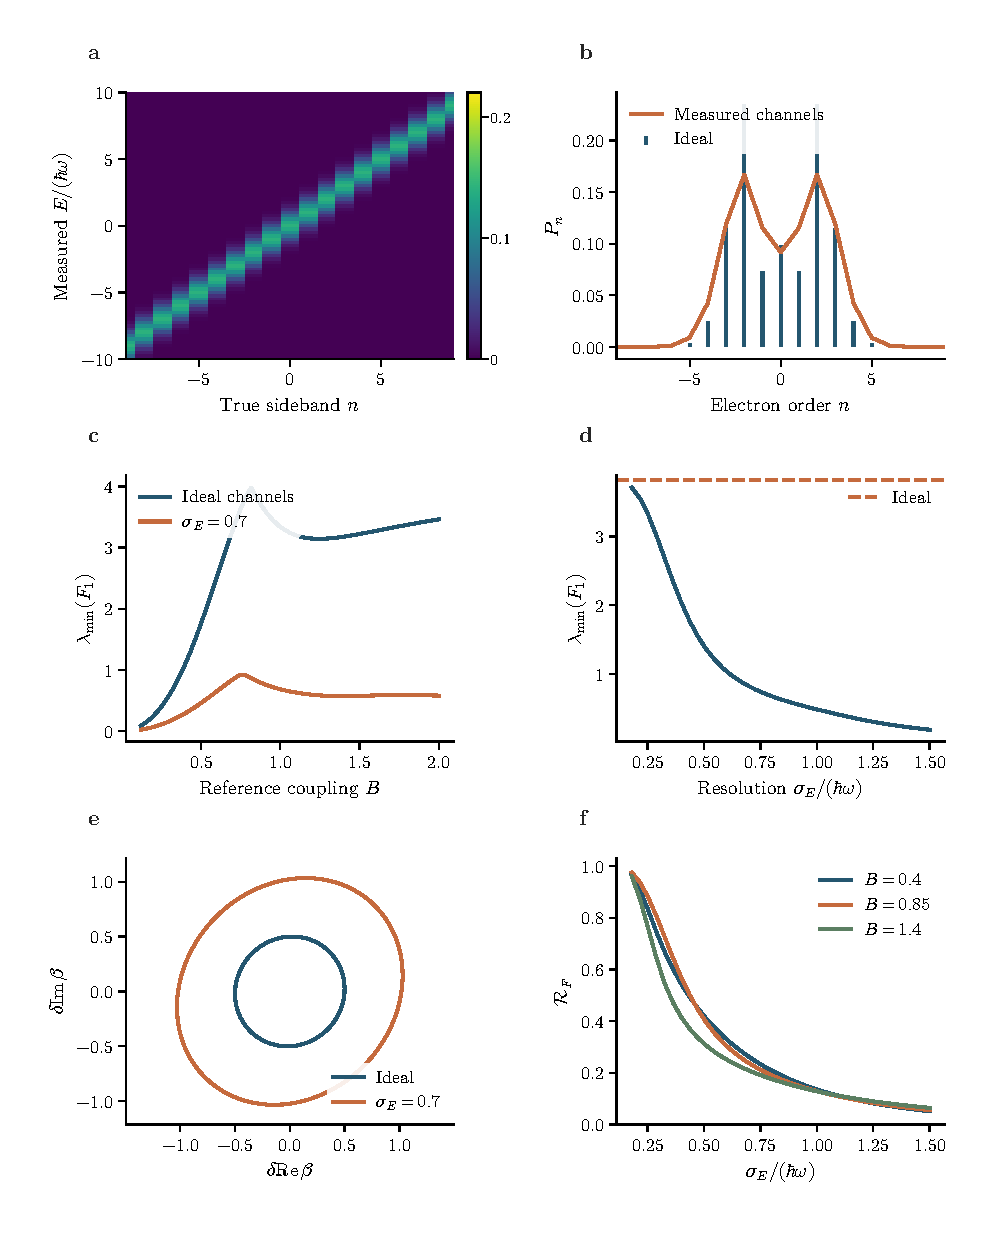
\includegraphics[width=0.96\linewidth,height=0.70\textheight,keepaspectratio]{phase_reference_information.pdf}
\caption{\textbf{相位反演的分辨率与 Fisher 信息预算。} (a) 真实能量边带与测得能量像素之间的高斯响应矩阵；(b) 理想离散边带与卷积后按单位边带宽分箱的观测概率，二者用同一概率单位比较；(c) 对复耦合两个分量的单位电子 Fisher 最小本征值随参考强度的变化；(d) 最小本征值随能量分辨率的下降及理想探测基准；(e) 单位电子局域 Fisher 协方差的两种误差椭圆，实测剂量 $N_e$ 下应将轴长同时除以 $\sqrt{N_e}$；(f) 不同参考幅值下，面积意义上的相对信息效率 $\mathcal R_F=\sqrt{\det F_{\rm det}/\det F_{\rm ideal}}$。图 (b) 将观测连续能量重新按宽度为一个光子能量的通道积分，因此没有混合概率质量与概率密度。}
\label{fig:phase-reference-information}
\end{figure}

数值实现中，真值继续采用 $x=0.67$、$y=0.46$ 和 $B=0.85$，设置 $n=-15,\ldots,15$。探测能量像素中心为 $u_j=-18,-17.75,\ldots,18$，单像素宽 $\Delta u=0.25$；响应矩阵 $R_{jn}$ 用\cref{eq:phase-reference-response-kernel} 的高斯积分，即正态分布累积分布函数在相邻像素边界之差计算，按真实边带列归一。(a) 使用 $s=0.7$ 绘制该矩阵，仅展示 $-9\le n\le9$ 与 $-10\le u\le10$ 的中心部分，色标是单个记录通道的条件概率；(b) 在参考相位 $\phi_r=0$ 比较理想 $P_n$ 与经过 $s=0.7$ 模糊后再按 $[n-1/2,n+1/2]$ 整合的能量通道概率，二者均是无量纲概率；(c) 参考幅值 $B\in[0.12,2.0]$ 取 55 点，分别用 $R=I$ 的理想离散边带及 $s=0.7$ 的模糊记录计算单位电子 $F_1=F/N_e$ 的最小本征值；(d) 固定 $B=0.85$，扫描 $s\in[0.18,1.5]$ 共 37 点，比较 $\lambda_{\min}(F_1)$ 与理想读出；(e) 比较 $F_1^{-1}$ 所给的单位电子误差椭圆，实际总剂量 $N_e$ 下轴长应按 $N_e^{-1/2}$ 缩放；(f) 对 $B=0.4,0.85,1.4$ 计算 $\mathcal R_F=\sqrt{\det F_{1,\mathrm{det}}/\det F_{1,\mathrm{ideal}}}$。数值导数采用解析的 $4J_n(2g)J_n'(2g)$，四参考相位分配等量剂量，零概率分母用 $10^{-13}$ 防止浮点下溢；这里不额外加入读出背景、效率漂移或光学参考校准误差。


两组图表明，\emph{反演是否无偏}与\emph{反演是否精确}是两个不同问题。稳定高斯展宽使四相位谱矩差分仍然无偏，但减少了完整测量数据的局域 Fisher 信息；即使均值关系可以消去共同偏置，读出噪声和有限统计仍使误差增长。若存在相位相关漂移、参考幅值未标定或非高斯响应，这种简单差分不再具备上述保证，必须把额外参数引入联合似然。

对于能量--OAM 联合读出，为什么增加一个坐标会提高某些参数的可辨识性，也能严格证明。设联合概率为 $p(N,L\mid\vb{\theta})=p_E(N\mid\vb{\theta})p(L\mid N,\vb{\theta})$。对数似然的导数分成能量边际的得分与条件 OAM 得分；条件得分在固定 $N$ 下平均为零，因此交叉项消失，得到
\begin{equation}
F_{NL}=F_E+\sum_N p_E(N)F_{L\mid N},\qquad F_{L\mid N}\succeq0.
\label{eq:oam-fisher-decomposition}
\end{equation}

这条信息分解关系值得从概率定义逐行证明，因为它说明增加 OAM 标签的收益究竟来自哪里，而不是依赖“二维图像更丰富”的直觉。为使符号明确，令 $p_{NL}(\vb\theta)>0$ 为归一化联合概率，边缘概率
$p_N=\sum_Lp_{NL}$，条件概率 $r_{L|N}=p_{NL}/p_N$。对任意待估参数 $\theta_a$，联合对数似然的导数（得分）满足
\begin{align*}
 s_a(N,L)&\equiv\partial_a\log p_{NL}
 =\partial_a\log p_N+\partial_a\log r_{L|N}\\
 &\equiv s_a^E(N)+s_a^{L|N}(L).
\end{align*}
这一步只使用了概率乘法公式，没有假设两个坐标统计独立。将得分的乘积按 $p_{NL}=p_Nr_{L|N}$ 取平均，得到四项，其中两个交叉项形如
\begin{align*}
 &\sum_{N,L}p_Nr_{L|N}s_a^E(N)s_b^{L|N}(L)\\
 &\qquad=\sum_Np_Ns_a^E(N)
   \underbrace{\sum_Lr_{L|N}\partial_b\log r_{L|N}}_{\displaystyle
   \sum_L\partial_b r_{L|N}=\partial_b1=0}=0.
\end{align*}
反向交叉项同样为零；所以剩余两项恰好是能量边缘的信息和条件 OAM 信息，得到\cref{eq:oam-fisher-decomposition}。

实验探测器会把这个理想信息再损失一部分。令 $R_{j,NL}$ 表示给定真实通道 $(N,L)$ 后记录为事件 $j$ 的条件概率，且假设它在参数范围内已标定并且不依赖未知的 $\vb\theta$。将真实通道合并为索引 $i$，写 $q_j=\sum_iR_{ji}p_i$，则记录端的得分是
\begin{align*}
 \partial_a\log q_j
 &=\frac{\sum_iR_{ji}\partial_a p_i}{q_j}
 =\sum_i\underbrace{\frac{R_{ji}p_i}{q_j}}_{P(i|j)}
 \partial_a\log p_i\\
 &=\mathbb E[s_a(i)\mid j].
\end{align*}
最后一行等于真实得分对所记录事件的条件平均。因此，对任意实向量 $\vb u$，条件方差非负给出
\begin{align*}
 \vb u^{\mathsf T}(F_{\mathrm{ideal}}-F_{\mathrm{det}})\vb u
 &=\mathbb E\!\left[(\vb u\cdot\vb s)^2\right]
 -\mathbb E\!\left[
   \mathbb E(\vb u\cdot\vb s\mid j)^2\right]\\
 &=\mathbb E\!\left[\operatorname{Var}(\vb u\cdot\vb s\mid j)\right]
 \ge0.
\end{align*}
于是得到了比单参数比较更强的矩阵不等式
\begin{equation}
 F_{\mathrm{det}}\preceq F_{\mathrm{ideal}}.
 \label{eq:detector-fisher-contract}
\end{equation}
这就是探测器模糊不能凭空增加经典 Fisher 信息的直接证明。证明要求固定的、与待估参数无关的随机响应；倘若改变实验设置同时改变了物理相互作用或测量基，比较的是两个不同的测量方案，就不能把这种变化当作简单的随机后处理。若存在探测效率损失，要么把未探测事件纳入 $j$，要么同时追踪总有效剂量；若总剂量本身依赖未知参数，还要保留总计数携带的信息。

这是一条关于理想同源数据的数学结论：对同一入射样本，保留更多事件标签不会降低经典 Fisher 信息，但新增信息也可能只沿已经灵敏的参数方向累积。若探测器 OAM 串扰只提供随机化而不携带参数信息，响应矩阵会再按数据处理不等式减少这份增益。

以两色调制的独立路径概率作为可计算基准，令
\begin{equation}
p(n_1,n_2)=J_{n_1}^2(2g_1)J_{n_2}^2(2g_2),\qquad
N=n_1+2n_2,\quad L=n_1-n_2.
\label{eq:oam-fisher-bessel-benchmark}
\end{equation}
理想联合测量保留 $p(N,L)$，而能量单独测量求和 $p_E(N)=\sum_Lp(N,L)$。这个路径概率只含两种调制强度 $g_1,g_2$，不含相对光学相位。因而它适合演示联合标签对两个强度参数的贡献，却不能用于宣称仅靠这种人口读出就可反演相位。若需要同时估计 $\phi=\arg\beta_2-2\arg\beta_1$，必须让原本可区分的路径在参考干涉或测量基旋转后相干叠加，使输出概率的导数 $\partial_\phi p$ 真正不为零。此时 Fisher 矩阵是否满秩，需要按实际响应重新计算，而不能仅凭二维图像更丰富就下结论。


总计数增加时，纯泊松统计误差通常按 $N^{-1/2}$ 缩小；校准偏差、模型误差和分辨率误差却不会自动随 $N$ 消失。因此达到系统误差地板以后，继续增加剂量可能几乎没有收益。

多参数实验设计也不能只最大化一个任意的 Fisher 标量。最大化 $\det F$（D-最优）倾向于缩小总体误差椭球体积；最大化最小本征值（E-最优）强调最难估计方向；最小化 $\operatorname{Tr}F^{-1}$（A-最优）强调平均方差。选择哪一个目标，取决于实验真正关心的是总体体积、最坏方向还是某个特定参数。图中的 $\operatorname{Tr}F$ 或其他简化分数只能作为特定设计准则，不能称为普适最优性。


先看只有两个观测通道的最小例子。设参数为 $\theta$，理想概率为 $q_1(\theta)=\theta$、$q_2(\theta)=1-\theta$，总计数为 $N$。代入\cref{eq:ch07-2}，有


\begin{equation*}
F(\theta)=N\left[\frac{1}{\theta}+\frac{1}{1-\theta}\right]=\frac{N}{\theta(1-\theta)}.
\end{equation*}


于是任何局部无偏估计都满足


\begin{equation*}
\operatorname{Var}(\hat\theta)\ge \frac{\theta(1-\theta)}{N}.
\end{equation*}


这个简单结果把三件事分开了。计数增加时误差按 $N^{-1/2}$ 缩小；概率对参数越敏感，Fisher 信息越大；若探测器模糊使两个不同 $\theta$ 产生更相近的观测分布，$\partial q_j/\partial\theta$ 变小，信息就会下降。后面的分辨率和最优设计图只是把这个计算推广到多通道、多参数和真实响应矩阵。

Fisher 矩阵在局部参数空间中给出一个二次型 $\dd s^2=\dd \vb{\theta}^{\mathsf T}F\,\dd \vb{\theta}$。若两个参数扰动产生相同的数据变化方向，这个二次型沿某个方向很小，误差椭圆就被拉长。最小本征值对应最难区分的参数组合，最大本征值对应最敏感方向。

因此“可辨识”首先是秩问题，其次才是精度问题。满秩但条件数很大表示理论上可区分、实际上需要大量计数；秩亏则表示仅靠当前测量无论增加多少重复次数都不能在局部一阶上分开参数。改变波长、偏振、参考相位或探测基的价值，就在于改变 $J$ 的列方向。


高信号并不一定代表高信息，低统计方差也不一定代表低总误差。若前向模型有系统偏差，或后验分布本身多峰，只报告局部 Fisher 下界会过于乐观。实验设计应同时检查前向模型、统计波动和模型误差。

\begin{figure}[!htbp]
\centering
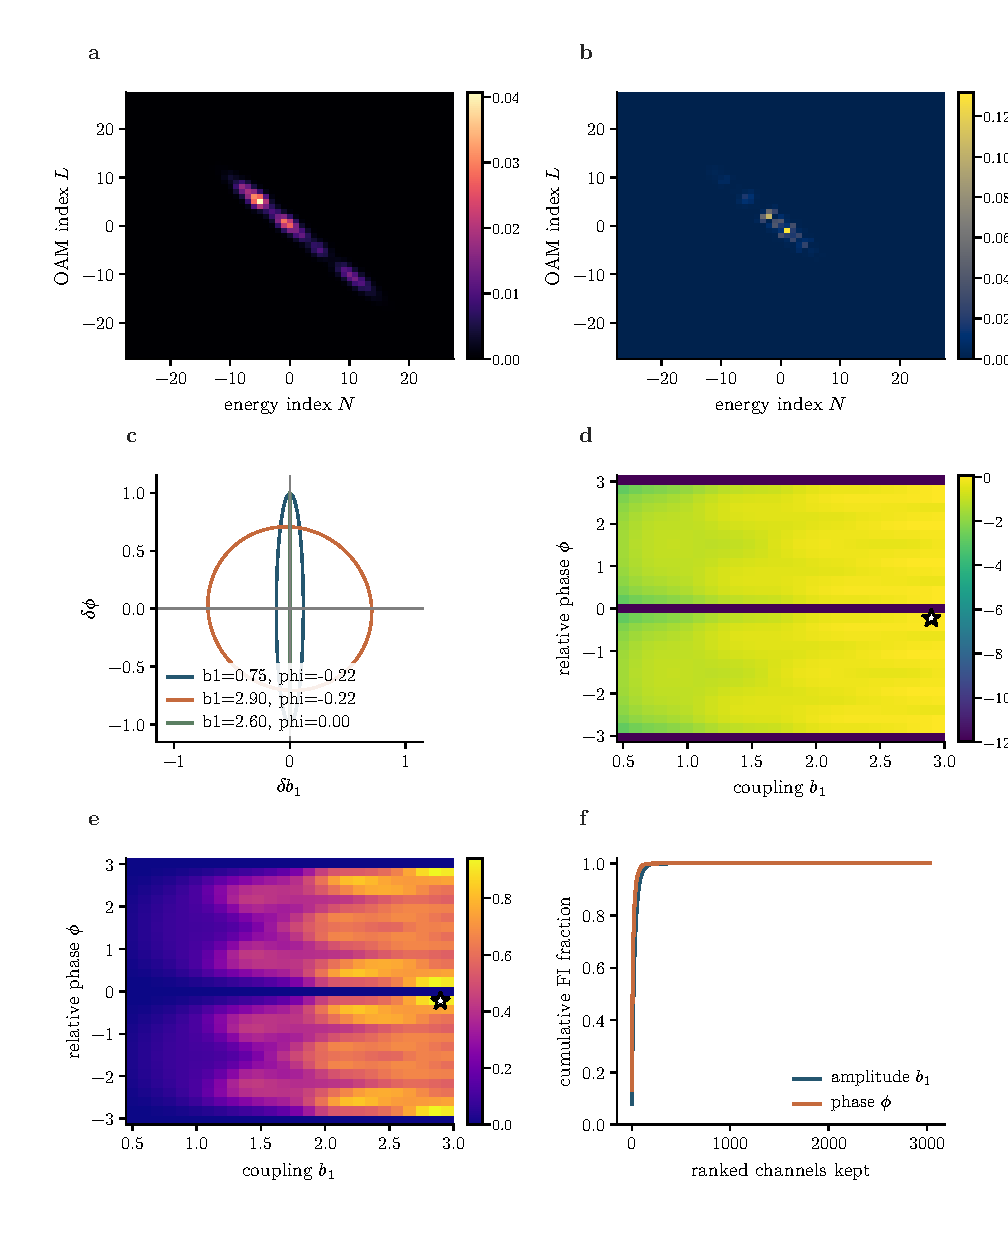
\includegraphics[width=0.96\linewidth,height=0.70\textheight,keepaspectratio]{fisher_geometry.pdf}
\caption{\textbf{Fisher 几何中的最优工作点、误差椭圆与信息预算}\quad 以两色 PINEM 的联合能量--OAM 计数分布 $q_{NL}(b_1,\phi)$ 为前向模型，取待估参数为耦合强度 $b_1$ 与相对相位 $\phi$。上排先给出鲁棒工作点处的联合响应与按通道分解的相位 Fisher 信息预算 $I^{(\phi)}_{NL}=(\partial_\phi q_{NL})^2/q_{NL}$，再比较三个工作点的局部误差椭圆。下排则在 $(b_1,\phi)$ 平面上画出 $\log_{10}\det F$ 与 $\lambda_{\min}(F)$：前者衡量总体信息体积，后者更直接刻画最差可辨识方向，从而选出对参数退化最不敏感的鲁棒工作点。最后一格把各通道按贡献排序，显示 Fisher 信息预算集中在少数最敏感的联合边带上。}
\label{fig:ch07-story-extensions--38-fisher-geometry}
\end{figure}

数值实现中，以两色 PINEM 的模糊联合分布 $q_{NL}(b_1,\phi)$ 为前向模型，其中第二色固定 $b_2=1.8$、轨道角动量步长取 $(\ell_1,\ell_2)=(-1,-2)$，能量与 OAM 探测器模糊核均取高斯宽度 $\sigma_N=\sigma_L=0.85$，边带截断 $n_{\max}=9$。对参数向量 $\vb{\theta}=(b_1,\phi)$，二维 Fisher 矩阵按
\[F_{ij}(\vb{\theta})=\sum_{N,L}\frac{1}{q_{NL}(\vb{\theta})}\frac{\partial q_{NL}}{\partial \theta_i}\frac{\partial q_{NL}}{\partial \theta_j},\qquad \theta_1=b_1,\ \theta_2=\phi,\]
计算；数值导数使用中心差分，步长分别为 $\delta b_1=0.035$、$\delta\phi=0.045$。参数扫描范围 $b_1\in[0.45,3.0]$（26 点）、$\phi\in[-\pi,\pi]$（29 点）。鲁棒工作点按 $\lambda_{\min}(F)$ 最大原则选取；在当前离散网格上得到 $b_1\approx2.90,\phi\approx-0.22$。误差椭圆由协方差近似 $C=F^{-1}$ 生成，为便于比较形状，在图中再除以 $\sqrt{\operatorname{Tr}\,C}$ 做无量纲归一。最后一格的信息预算曲线把各像素对 $F_{11}$ 与 $F_{22}$ 的贡献
\[I^{(b_1)}_{NL}=\frac{(\partial_{b_1}q_{NL})^2}{q_{NL}},\qquad I^{(\phi)}_{NL}=\frac{(\partial_{\phi}q_{NL})^2}{q_{NL}}\]
按从大到小排序并做累计和，直接显示“最有用的通道”占总信息的比例。


\medskip
参数约束来自计数似然，而非理想谱的形状；后面的算例同时展示探测响应、局域信息与统计反演，以区分随机误差和模型偏差。


\medskip
任何反演都必须先写前向模型：真实边带人口经过有限分辨率、效率和背景后才成为实验计数，因此直接对理想谱拟合会产生系统偏差。

对独立泊松计数，Fisher 矩阵由期望计数对参数的导数组成；其秩、最小本征值和条件数决定多参数问题是否局域可辨识，而不是由某一条谱线是否足够强决定。

Cramér--Rao 下界是无偏估计量的局域频率学界限；贝叶斯后验还包含先验信息，因此后验收缩不能简单等同于数据本身的 Fisher 信息增加。

实验设计应同时考虑统计方差、模型偏差和参数退化；D/E/A 最优等准则回答不同问题，不能把单一的 $\operatorname{Tr}F$ 当成普适最优目标。低能 Bragg 区的二能级电子进一步提供了一个干净基准：可以直接把 Rabi/Ramsey 条纹的可见度、泄漏和单位剂量 Fisher 信息放在同一前向模型中比较。

至此，近场动力学、传播、合成维度、量子光、开放系统和多体关联都已经与实际计数模型接通。进一步比较模型的适用边界时，应当从已经写入探测器响应的完整前向链条出发，检查某个近似所丢失的自由度是否已经影响可测计数。


这些局部信息量最终还须经过一次端到端的检验：从近场模型生成边带，经探测器得到含泊松涨落的计数，再\emph{只凭这些计数}反推原始参数。\cref{fig:ch07-inverse-problem} 把这一过程计算到底，避免把“图像看得见”和“参数能被无偏反演”混为一谈。这里的近场横向形状是解析的高斯代理，而不是对某种实际纳米颗粒的未经标定的材料预测。

\begin{figure}[!htbp]
\centering
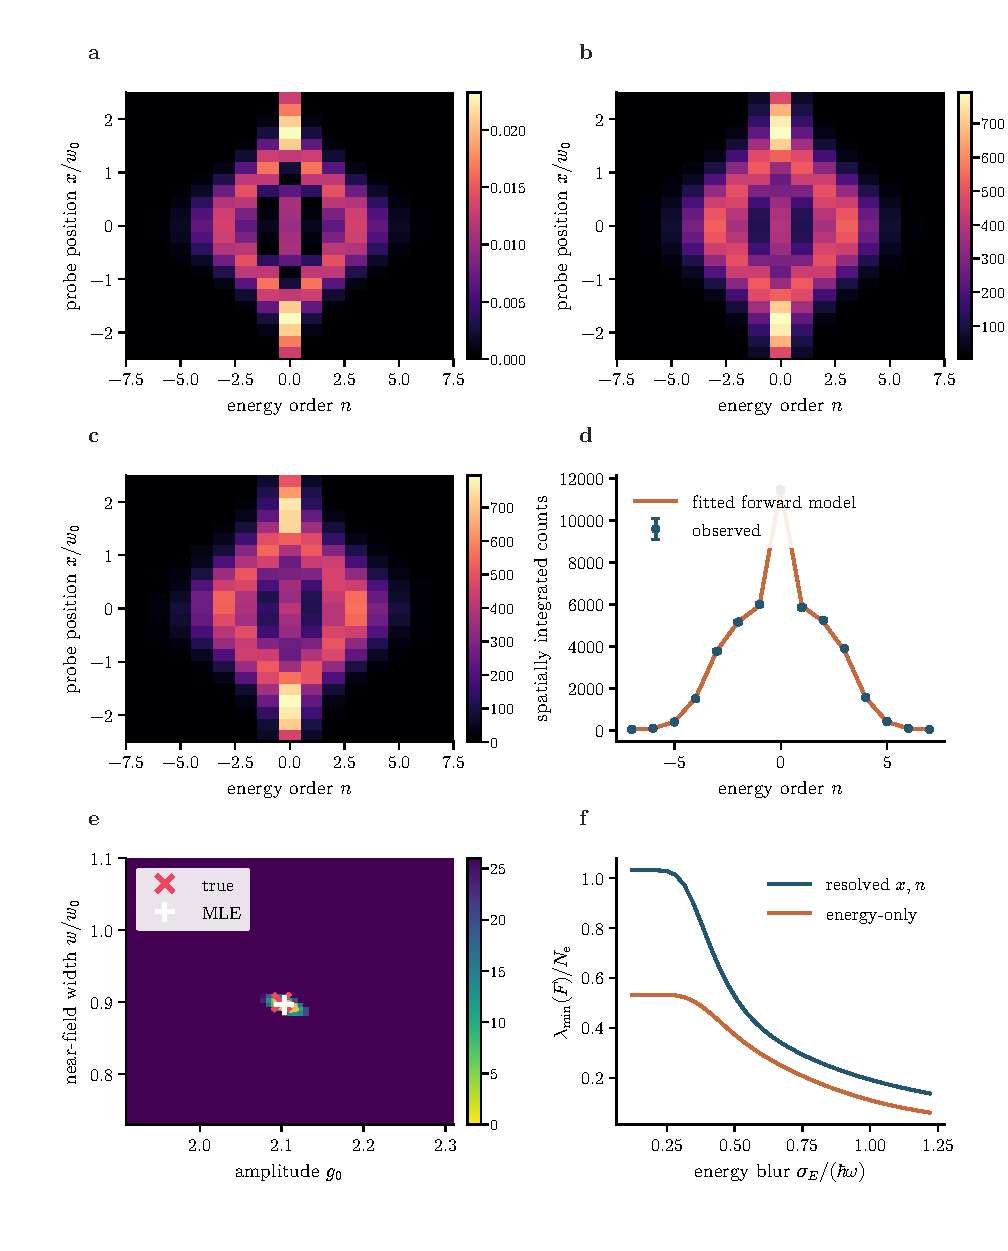
\includegraphics[width=0.97\linewidth,height=0.70\textheight,keepaspectratio]{detector_inverse_problem.pdf}
\caption{\textbf{从可控近场模型到实验计数与双参数反演。} (a) 峰值和横向宽度决定理想空间--能量联合概率；(b) 对同一分布卷积探测器空间/能量响应，并加入有限剂量和已知均匀背景；(c) 由各像素独立的泊松抽样形成一次实际数据；(d) 把同一数据的能量边际与联合最大似然模型的预测直接比较；(e) 放大最优点附近的两参数似然，标出真实参数与网格最大似然估计及二维渐近置信轮廓；(f) 比较保留全部空间--能量通道与只保留能量边际时的 Fisher 最小本征值，说明增加测量坐标何时真正改善最差可辨识方向。}
\label{fig:ch07-inverse-problem}
\end{figure}

数值实现中，\par\smallskip
全部长度与能量用无量纲单位，规定横向耦合 $\beta(x)=g_0\exp[-x^2/(2w^2)]$，真值为 $g_0=2.1$、$w=0.90$。在 $x\in[-2.4,2.4]$ 的 23 个像素和 $n=-7,\ldots,7$ 的 15 个能量通道上，入射强度权重与理想联合概率为
\[
W_j=\frac{e^{-x_j^2/(2\sigma_b^2)}}{\sum_r e^{-x_r^2/(2\sigma_b^2)}},\ \sigma_b=1.30,\qquad
Q_{jn}=\frac{W_jJ_n^2(2\beta(x_j))}{\sum_{r,m}W_rJ_m^2(2\beta(x_r))}.
\]
探测器能量与空间响应分别取\emph{按真值通道列归一}的高斯矩阵
\[
K^{(E)}_{nm}=\frac{e^{-(n-m)^2/(2\sigma_E^2)}}{\sum_\ell e^{-(\ell-m)^2/(2\sigma_E^2)}},\qquad
K^{(x)}_{jr}=\frac{e^{-(x_j-x_r)^2/(2\sigma_x^2)}}{\sum_s e^{-(x_s-x_r)^2/(2\sigma_x^2)}},
\]
固定 $\sigma_E=0.48$（单位 $\hbar\omega$）与 $\sigma_x=0.25$（同一 $x$ 坐标单位）。(a) 为 $Q$；(b) 以 $N_e=45000$、每个测量像素的已知背景 $b=1.5$ 计算期望计数
\[
\mu_{jn}=N_e(K^{(x)}Q[K^{(E)}]^\mathsf T)_{jn}+b;
\]
(c) 在每个测量通道独立取 $Y_{jn}\sim\mathrm{Poisson}(\mu_{jn})$，随机种子 $27$；(d) 沿空间指标 $j$ 求和，将实际计数与双参数最大似然模型的能量边际比较，误差棒为 $\sqrt{\sum_jY_{jn}}$；(e) 使用 $g_0\in[1.91,2.31]$、$w\in[0.73,1.10]$ 各 61 点的局部参数网格，绘制
\[
-\ln\mathcal L(g_0,w)=\sum_{jn}[\mu_{jn}(g_0,w)-Y_{jn}\ln\mu_{jn}(g_0,w)]+\mathrm{const}
\]
的 $2\Delta(-\ln\mathcal L)$，并画 $2.30$ 和 $6.18$ 两条常用二维渐近置信等值线（不保证有限样本精确覆盖率）；该模型的一次模拟中拟合结果近似为 $(\hat g_0,\hat w)=(2.11,0.89)$。(f) 在 $\sigma_E\in[0.12,1.22]$ 的 35 点上计算
\[
F_{ab}=\sum_{jn}\frac{(\partial_a\mu_{jn})(\partial_b\mu_{jn})}{\mu_{jn}},\quad a,b\in\{g_0,w\},
\]
并显示 $\lambda_{\min}(F)/N_e$；数值导数用 $0.008$ 的中心差分。仅测能量时，把空间像素计数先求和，相应背景为 $23b$，然后重新求同一双参数 Fisher 矩阵。这里没有加入额外的材料标定不确定度或统计先验。


图 (e) 的倾斜置信轮廓来自峰值耦合与有效作用宽度之间的参数关联：二者都能扩展边带，但对空间分布造成的变化并不相同。图 (f) 因此也不是“多一个探测维度必然更好”的普遍宣言，而是在明确的响应矩阵、噪声和两个待估参数之下，检验联合读出是否保留了新的、线性独立的灵敏度方向。

\clearpage
\par\medskip 在合成维度章节的可逆能量--OAM 映射中，每个 $ (N,L)$ 通道对应唯一 $(n_1,n_2)$，理想联合\emph{人口}只包含各贝塞尔权重的乘积，相对光学相位被模平方消去。本章为了演示“由路径干涉提取相位”，刻意采用 $\ell_2=2\ell_1$ 的退化映射，让不同路径到达同一输出；它牺牲路径可区分性，却使人口测量拥有非零相位 Fisher 信息。要同时兼得路径解码和相位估计，必须额外引入参考臂、输出干涉或改变测量基。


\noindent \figref{fig:ch07-story-extensions--38-fisher-geometry}：六面板计算逐项核对。\par\noindent (a) 在鲁棒工作点 $(b_1,\phi)\approx(2.90,-0.22)$ 直接绘制模糊联合分布 $q_{NL}$；(b) 对同一点计算相位信息密度 $I^{(\phi)}_{NL}=(\partial_\phi q_{NL})^2/q_{NL}$；(c) 比较三组工作点 $(0.75,-0.22)$、$(2.90,-0.22)$ 与 $(2.60,0)$ 的协方差椭圆，均使用 $C=F^{-1}$，再用 $\sqrt{\operatorname{Tr}\,C}$ 归一化只保留形状与朝向；(d) 在 $26\times29$ 的 $(b_1,\phi)$ 网格上绘 $\log_{10}\det F$，星号标出最优工作点；(e) 在同一网格上绘 $\lambda_{\min}(F)$，它是文中用来定义“鲁棒工作点”的主准则；(f) 对最优工作点把所有像素的 $I^{(b_1)}_{NL}$ 与 $I^{(\phi)}_{NL}$ 排序后求累计和，显示前少量通道已经占据几乎全部 Fisher 预算。整个图中 $q_{NL}$ 始终保持归一化，差分导数不再单独加噪声或后验先验；因此这是一张基于前向模型与探测模糊核的局部可辨识性分析图。

\par\medskip
由同一个计数似然得到 Fisher 信息和后验分布之后，还必须检验建立该似然的动力学模型是否适用。不同能量、波包尺寸、光场统计和探测分辨率会要求不同的理论层级；因此最后回到最小耦合哈密顿量，明确何时需要升级模型。
\par\medskip


此前已经建立了相对论正能输运、经典 PINEM、精确近场散射、纵向相空间、合成维度、量子光、开放系统、多电子关联和测量反演等不同层级的模型。这些模型并不是彼此独立的工具箱；它们来自同一套电子--电磁场动力学，只是在不同尺度下保留了不同自由度。

要判断某个实验应使用哪一级理论，必须从基本哈密顿量出发，沿近似链追踪被保留和被舍弃的自由度，并最终闭合到探测器计数。本章把前面的模型放回同一条理论链，并给出每一级模型的控制参数与失效条件。


\section{模型适用边界}
为了判断前面哪一种模型适合新的实验，需要回到未约化的电子—电磁场哈密顿量。不同章节的公式并不互相竞争，而是对同一动力学保留不同自由度之后的结果。

对电荷 $-e$ 的非相对论电子，最小耦合哈密顿量写成
\begin{equation}
H=\frac{[\vb{p}+e\vb{A}(\vb{r},t)]^2}{2m}-e\phi(\vb{r},t)
=\frac{\vb{p}^2}{2m}+H_{pA}+H_{A^2}-e\phi,
\label{eq:ch08-minimal}
\end{equation}
其中
\begin{equation}
H_{pA}=\frac{e}{2m}(\vb{p}\cdot\vb{A}+\vb{A}\cdot\vb{p}),
\qquad
H_{A^2}=\frac{e^2\vb{A}^2}{2m}.
\label{eq:ch08-interactions}
\end{equation}
在高能电子、窄动量包络中，可以围绕中心动量 $p_0$ 线性化电子色散；在低能 Bragg 区，二阶色散反而必须保留，因为它负责把非目标边带失谐。近场耦合章节和合成维度章节看似使用不同哈密顿量，本质上只是对同一个自由电子色散采用了不同截断。

这里必须强调规范问题。$H_{pA}$ 与 $H_{A^2}$ 的分拆本身不是可观测量；规范变换会重新分配中间项。若研究目标涉及二阶光场过程，必须在给定规范中保留同一微扰阶数的所有贡献，或者直接使用规范不变的散射振幅。把某个中间项单独称为“可测的两光子机制”之前，应先证明最终概率不依赖规范选择。

当电子偏折小、反冲小、横向位置在作用区内近似固定时，电子可以沿 $z=vt$ 的未扰轨迹积累相位。对单色纵向电场得到
\begin{equation}
\beta(\vb{R})=\frac{e}{2\hbar\omega}\int \dd z\,E_z(\vb{R},z)\ee^{-\ii\omega z/v}.
\label{eq:ch08-beta}
\end{equation}
这一步同时做了三件事：把三维场压成轨迹 Fourier 分量；把作用时间换成空间积分；把复杂材料电动力学对电子的影响压进一个复数。只要横向波包足够窄，$\beta(\vb{R})$ 还可以进一步用束心值近似。

得到 $\beta$ 后，经典场电子幺正算符可以写成能量平移算符的位移型形式
\begin{equation}
U_e(\beta)=\exp(-\beta b^\dagger+\beta^*b),
\qquad b|n\rangle=|n-1\rangle.
\label{eq:ch08-electron-displacement}
\end{equation}
这里沿用前文已经固定的能量升降算符约定：$b|n\rangle=|n-1\rangle$，$b^\dagger|n\rangle=|n+1\rangle$。在理想无限阶梯上 $bb^\dagger=b^\dagger b=1$；有限截断时需另行处理边界，不能直接将截断后的平移算符视为幺正。对初始能量本征态作用并展开，就得到
\begin{equation}
\langle n|U_e(\beta)|0\rangle
=J_n(2|\beta|)\ee^{\ii n\arg(-\beta)},
\label{eq:ch08-bessel}
\end{equation}
所以贝塞尔函数不是经验拟合，而是平移算符指数的 Fourier 系数。

一旦电子与光场的交换不再由确定的经典复振幅刻画，最小耦合模型便需要把光子自由度重新纳入 Hilbert 空间。经典结果必须能够作为这一联合理论的大光子数极限出现。
若单个光学模式必须量子化，最小有效联合幺正算符是
\begin{equation}
U_{e\gamma}(g)=\exp(g a^\dagger b-g^*b^\dagger a).
\label{eq:ch08-quantum-pinem}
\end{equation}
它把“电子下降一个能量格点、光子增加一个”与其逆过程成对写入，因此自动守恒总交换能量。若光场处于大振幅相干态 $|\alpha\rangle$，且电子对场的相对回作用很小，可在平均场层面令 $a\to\alpha$，于是
\begin{equation}
U_{e\gamma}(g)\longrightarrow
\exp(g\alpha^* b-g^*\alpha b^\dagger)
=U_e(\beta),
\qquad \beta=g^*\alpha.
\label{eq:ch08-classical-limit}
\end{equation}
这里的等号采用 $U_e=\exp(-\beta b^\dagger+\beta^*b)$ 的相位约定；若改用相反方向的能量平移或不同的相互作用相位定义，$\beta$ 的复共轭与整体负号会相应改变，但边带概率仍由 $|\beta|$ 决定。比较复振幅时必须保持同一约定。

如果输入不是相干态，不能把 $a$ 替成一个数。光子数态矩阵元含有 $\sqrt N$，所以不同 $p_N$ 即使有相同 $\bar N$ 也会给出不同电子谱。若最终只测电子，必须做偏迹
\begin{equation}
\rho_e'=\operatorname{Tr}_\gamma\!
\left[U_{e\gamma}(\rho_e\otimes\rho_\gamma)U_{e\gamma}^\dagger\right].
\label{eq:ch08-trace}
\end{equation}
若还测光子，联合概率保留更多信息；若先测电子并条件化光场，则得到 Kraus 算符
\begin{equation}
M_m=\langle m|U_{e\gamma}|\psi_e\rangle,
\qquad
\rho_{\gamma|m}=\frac{M_m\rho_\gamma M_m^\dagger}{\operatorname{Tr}(M_m\rho_\gamma M_m^\dagger)}.
\label{eq:ch08-kraus}
\end{equation}
量子光章节的电子后选择光场方案正是这类条件测量算符的一个物理实现。

理想 PINEM 把相邻能量格点视为等间隔，并假定跃迁失谐不随 $n$ 改变。保留相对论色散二阶项后，能量格点获得近似 $n^2$ 的额外相位/在位能。写成
\begin{equation}
H_{\rm lat}=\sum_n\left(n\hbar\omega+\chi n^2\right)|n\rangle\langle n|
+\sum_n(g|n+1\rangle\langle n|+\mathrm{h.c.}),
\label{eq:ch08-recoil-lattice}
\end{equation}
其中 $\chi$ 由电子色散和具体相位匹配决定。$\chi\to0$ 时恢复平移对称能量晶格；$|\chi|$ 与 $|g|$ 可比时，邻近通道逐渐失谐并进入 Bragg/二能级极限。因此高能 PINEM 和低能 Rabi 电子不是两个无关现象，而是同一个能量晶格在“跃迁带宽大于/小于反冲曲率”两侧的极限。


前面的 $\chi n^2$ 有效晶格式还没有直接告诉我们“二能级近似会错到什么程度”。最可靠的做法，是把二能级截断作为一个需要检验的近似，而不是把它定义成真理。为此选择旋转表象，使 $|0\rangle$ 和 $|1\rangle$ 正好在共振点简并。将自由色散的线性项吸收入驱动频率以后，最小多通道模型可写成
\begin{equation}
H_{\rm rot}=\chi\sum_{n\in\mathbb Z}n(n-1)|n\rangle\langle n|
+g\sum_n\bigl(|n+1\rangle\langle n|+|n\rangle\langle n+1|\bigr).
\label{eq:ch08-rotating-recoil}
\end{equation}
这里 $g,\chi$ 具有能量量纲，并且只针对旋转框架中一对选定通道近共振的模型。$n=0,1$ 的在位能同为零，邻近的 $n=-1,2$ 的失谐为 $2\chi$，因此在 $g\ll2|\chi|$ 时才有将其他阶微扰消去的控制参数。注意这一准则不是一般性地说“反冲越大越强”，而是相对于被选择的共振通道的\emph{非目标跃迁失谐}来判断。


二能级约化的控制参数可以从完整阶梯精确推导，而不是靠“第三条边带看不见”判断。设 $P=|0\rangle\langle0|+|1\rangle\langle1|$ 是目标子空间投影，$Q=1-P$，并将本征方程 $H|\Psi\rangle=E|\Psi\rangle$ 分别左乘 $P$、$Q$。当 $E-QHQ$ 在 $Q$ 子空间中可逆时，第二个方程给出
\begin{equation*}
Q|\Psi\rangle=(E-QHQ)^{-1}QHP\,P|\Psi\rangle.
\end{equation*}
将其代回第一个方程，得到能量依赖的精确约化本征方程
\begin{equation}
\Bigl[PHP+PHQ(E-QHQ)^{-1}QHP\Bigr]P|\Psi\rangle=E\,P|\Psi\rangle.
\label{eq:bragg-resolvent-effective}
\end{equation}
第二项称为自能。它保留了虚跃迁离开目标子空间再返回所积累的相位，因此即使 $Q$ 子空间的最终人口很小，也不能自动丢掉这项。记目标能量与非目标谱的最小距离为 $\Delta_{\mathrm{leak}}$，并要求 $\|PHQ\|/\Delta_{\mathrm{leak}}\ll1$，才可把 resolvent 按耦合展开。在不靠近 $QHQ$ 共振的区域，主要修正满足
\begin{equation}
\delta H_{\mathrm{eff}}=O\!\left(\frac{|g|^2}{\Delta_{\mathrm{leak}}}\right),\qquad
P_{\mathrm{leak}}=O\!\left(\frac{|g|^2}{\Delta_{\mathrm{leak}}^2}\right).
\label{eq:bragg-leakage-estimates}
\end{equation}
两个量的物理后果不相同：泄漏主要表现为目标双能级之外的计数，而自能修正经过持续时间 $T$ 还会积累量级 $|g|^2T/(\hbar\Delta_{\mathrm{leak}})$ 的相位偏差。后者可能在多余边带尚不可分辨时，已经移动了由 Rabi 条纹反演得到的耦合强度。这正是必须同时检查泄漏、保真度和条纹相位的原因。

对于非相对论自由电子，若一次交换纵向动量 $\hbar q$，则
\begin{equation}
E_n-E_0=\frac{(p_0+n\hbar q)^2-p_0^2}{2m_e}
=n\hbar qv_0+n^2E_R,\qquad E_R=\frac{\hbar^2q^2}{2m_e}.
\label{eq:bragg-recoil-from-dispersion}
\end{equation}
把共振框架的线性失谐调成 $-E_R$，即得到上式中的 $\chi=E_R$ 与在位能 $E_Rn(n-1)$。对相对论电子，色散的曲率由 $E''(p_0)=1/(\gamma^3m_e)$ 给出，二次项系数相应替换为 $(\hbar q)^2/(2\gamma^3m_e)$。该替换只在被占据动量宽度足以使三阶余项可忽略时成立；它不是把所有复杂三维散射误差一并吸收进一个“有效反冲能”的许可。

在严格二能级极限，初态 $|0\rangle$ 的波函数应为
\begin{equation}
|\psi_2(\tau)\rangle=\cos(g\tau)|0\rangle-\ii\sin(g\tau)|1\rangle,
\qquad \tau_{\pi/2}=\frac{\pi}{4g},
\label{eq:ch08-bragg-target}
\end{equation}
其中已经取 $\hbar=1$ 的计算单位。我们用同一个名义半 Rabi 脉冲时间作用于\cref{eq:ch08-rotating-recoil} 的完整有限阶梯，然后同时报告外泄和目标态保真度：
\begin{equation}
L=1-P_0(\tau_{\pi/2})-P_1(\tau_{\pi/2}),\qquad
\mathcal F=|\langle\psi_2(\tau_{\pi/2})|\psi_{\rm full}(\tau_{\pi/2})\rangle|^2.
\label{eq:ch08-leakage-fidelity}
\end{equation}
这两个误差不能混成一个数。$L$ 只询问概率是否泄漏到其他阶；即使 $L$ 很小，二能级子空间内部仍可能积累错误的相对相位，使 $\mathcal F$ 降低。对光学脉冲序列或量子逻辑门而言，后者正是实验中不可忽视的相干误差。

\begin{figure}[!htbp]
\centering
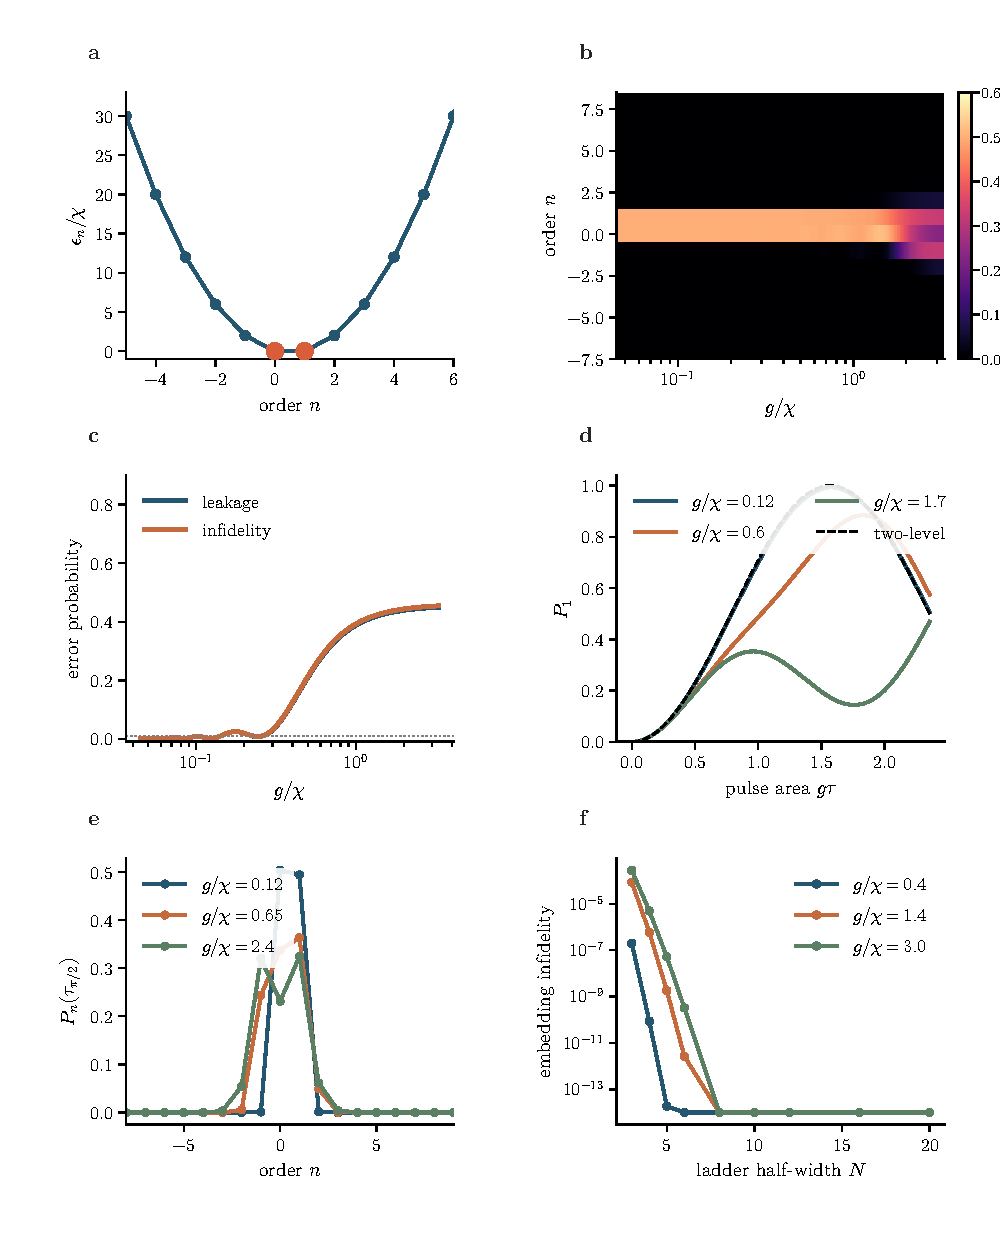
\includegraphics[width=0.97\linewidth,height=0.70\textheight,keepaspectratio]{recoil_transition.pdf}
\caption{\textbf{反冲区的二能级近似：从严格共振对到多边带失效}\quad (a) 旋转表象的二次在位能 $\chi n(n-1)$ 明确隔离 $n=0,1$ 一对共振态；(b) 保持名义半 Rabi 脉冲时间 $\tau_{\pi/2}=\pi/(4g)$ 不变时，随 $g/\chi$ 增大的终态人口扇形；(c) 非目标通道泄漏与目标态失保真并非同一误差；(d) 对照完整多阶梯的 $P_1(\tau)$ 与理想 $\sin^2(g\tau)$；(e) 不同耦合比下的完整输出能谱，直观看到目标态以外的新阶数；(f) 随有限能量截断 $N$ 变化的结果收敛性。六面板同时检查物理近似误差与数值截断误差，没有通过未声明的唯象线宽掩盖多通道效应。}
\label{fig:ch08-recoil-transition}
\end{figure}

最右下角的截断图常常比“漂亮的多边带热图”更重要，因为有限矩阵指数始终会给出形式上规范化的概率，但这并不保证边界没有污染动力学。若 $N$ 增大以后目标态保真度仍发生可观测变化，意味着曾经选择的数值 Hilbert 空间太小，不能将图像里的新峰解释为可靠物理。相反，只有当截断扫描稳定且不同近似计算指向同一极限，模型交叉区的定量阈值才值得用于实验设计。

一个方便的无量纲判断是
\begin{equation}
\mathcal R=\frac{|g|}{\Delta_{\rm rec}},
\label{eq:ch08-ratio}
\end{equation}
其中 $\Delta_{\rm rec}$ 表示相邻非目标通道由反冲产生的典型失谐。$\mathcal R\gg1$ 时多边带 Raman--Nath/PINEM 图像自然；$\mathcal R\ll1$ 且调到单一共振时二能级 Bragg 图像自然；$\mathcal R\sim1$ 正是模型边界章节提出的交叉区研究问题。

真正的实验还有未观测的声子、材料激发和光学模式；在量子模型中，它们不能简单视为一个随机相位，而必须通过偏迹与量子通道进入电子态。
若电子同时激发未被测量的材料模式、声子或其他光学通道，联合演化仍可幺正，但电子子系统不再幺正。一般量子通道写成
\begin{equation}
\mathcal E(\rho_e)=\sum_\mu K_\mu\rho_eK_\mu^\dagger,
\qquad \sum_\mu K_\mu^\dagger K_\mu=1.
\label{eq:ch08-channel}
\end{equation}
这里 $\mu$ 可以理解为环境中未读取的不同散射结果。若不同电子路径在环境中留下几乎正交的状态，路径非对角元会被压低；若环境无法区分两条路径，相干性可以保留。开放系统章节的 Lindblad 方程只是 Markov 极限下对这类通道的连续时间近似。

因此“退相干率”不应被当作随意加入的拟合常数。更物理的路线是先问环境有哪些模式、电子怎样耦合、哪些环境结果被迹掉，再决定是否可以压缩成少数 $\Gamma_j$。材料 Green 张量、损耗函数和局域态密度之所以重要，是因为它们给出了这些 $K_\mu$ 或连续谱率的微观来源。

实验从不直接“看到波函数”。给定最终联合态 $\rho$，一个测量设置 $x$ 对应 POVM $\{\Pi_y^{(x)}\}$，数据概率是
\begin{equation}
p(y|x,\theta)=\operatorname{Tr}[\Pi_y^{(x)}\rho(\theta)].
\label{eq:ch08-born}
\end{equation}
EELS 选择能量基；homodyne 型自由电子干涉选择相位敏感基；comb-basis 方案试图测量 $b_\Omega$ 的本征相位；OAM-EELS 进一步把测量扩展到能量--角动量联合基。所谓“一个新效应能否观察到”，最终必须翻译成两个竞争模型 $p_0(y)$ 与 $p_1(y)$ 在真实响应矩阵和噪声下是否可区分。

如果探测器响应为 $K_{jy}$、背景为 $b_j$、总剂量为 $N$，实验计数均值为
\begin{equation}
\mu_j(\theta)=N\sum_yK_{jy}p(y|\theta)+b_j.
\label{eq:ch08-detector}
\end{equation}
探测器卷积与背景可能显著改变参数可辨识性，因此理想概率中的大差异未必对应可分辨的计数信号。任何原创预测若没有走到\cref{eq:ch08-detector}，都还没有闭合到实验。


\begin{longtable}{p{0.16\linewidth}p{0.21\linewidth}p{0.22\linewidth}p{0.25\linewidth}}
\toprule
问题特征 & 最小模型 & 主要控制参数 & 失败时升级方向\\
\midrule
\endfirsthead
\toprule
问题特征 & 最小模型 & 主要控制参数 & 失败时升级方向\\
\midrule
\endhead
强相干经典光、高能电子 & $U_e(\beta)$ 与贝塞尔边带 & $|\beta|$、相位失配、$\epsilon_{\rm rec}$ & 三维 Floquet / 反冲晶格\\
光子统计可分辨 & $U_{e\gamma}(g)$ & $|g|$、$\bar N$、Fano 因子、损耗 & 多模 QED、联合测量\\
低能、反冲隔离两态 & 二能级 Bragg / Dirac & $|g|/\Delta_{\rm rec}$、失谐、波包宽度 & 多通道 TDSE/Floquet\\
材料激发造成相干损失 & Kraus/Lindblad & 哪一路可区分度、谱密度、传播时间 & 非 Markov 环境、显式材料模式\\
多电子同时参与 & 反对称两体态 + 相互作用 & 波包重叠、库仑能、可分辨性 & 多体散射/二次量子化\\
要估计未知参数 & POVM + 探测器前向模型 & Fisher 秩、条件数、系统误差 & 新测量基/新波长/联合探测\\
\bottomrule
\end{longtable}

检验一个自由电子量子光学模型时，可以依次追踪六件事：Hilbert 空间保留了哪些自由度、哪些自由度被经典化或迹掉；新效应由哈密顿量中的哪一项产生；模型是否存在明确的小参数并能在相应极限回到已知结果；理论图像对应波函数内部量、理想概率还是已经卷积探测器后的实验计数；结论是否依赖不可直接测的中间量以及如何排除替代解释；改变实验旋钮或交换操作次序后，是否出现低阶模型严格禁止的新信号。

只有当这六个问题能够从哈密顿量一直追踪到探测器计数，并且每一步近似的脆弱点都明确时，模型的适用范围才算真正闭合。

\par\medskip 从近场轨迹积分到量子联合态，再到环境偏迹和实验计数，前面所建立的模型可以按近似层级逐步升级。反冲交叉区的有限能量阶梯为这一层级提供了一个实用的数值检验：不只问模型能否解释图像，还要问最小截断、物理近似与最终观测的三种误差是否彼此一致。

\par\medskip

\noindent \figref{fig:ch08-recoil-transition} 的计算与截断。
所有面板均使用\cref{eq:ch08-rotating-recoil}，以 $\chi=1$ 作为能量单位，在初始 $|0\rangle$ 上演化；默认有限阶梯 $n=-12,\ldots,12$，仅有最近邻跃迁且统一 $g\in\mathbb R_+$。(a) 在 $n=-5,\ldots,6$ 上画二次在位能 $n(n-1)$，红色标记 $n=0,1$；(b,c) 在 $g/\chi\in[0.045,3.3]$ 的 95 个对数均匀点上，均取 $\tau=\pi/(4g)$ 并计算 $P_n=|[\ee^{-\ii H_{\rm rot}\tau}]_{n0}|^2$；(b) 显示 $n=-7,\ldots,8$，色阶上限为 $0.6$，(c) 分别计算\cref{eq:ch08-leakage-fidelity} 中的 $L$ 和 $1-\mathcal F$。(d) 分别取 $g/\chi=0.12,0.6,1.7$，在 $0\le g\tau\le3\pi/4$ 上各采 150 点，画 $|\langle1|\ee^{-\ii H\tau}|0\rangle|^2$ 和理想 $\sin^2(g\tau)$；(e) 对 $g/\chi=0.12,0.65,2.4$ 展示 $\tau_{\pi/2}$ 处的 $P_n$。(f) 固定 $g/\chi=0.4,1.4,3.0$，分别将半宽度截断 $N=3,4,5,6,8,10,12,16,20$ 的态嵌入到参考 $N=32$ 的空间，计算 $1-|\langle\psi_{32}|\psi_N\rangle|^2$；显示下限截为 $10^{-14}$ 以避免有限精度取对数发散。整个模型未加入衰减、脉冲包络或材料损耗；因此它只检验受控二次失谐和数值截断，不替代真实有限作用区下的完整三维 Floquet 散射。


当横向尺寸与入射束腰相当，或入射电子不能再当作沿固定直线传播的慢变包络时，简单的 $\beta$ 近似会漏掉不同横向散射通道的干涉。回到时周期哈密顿量，可以在保留多通道边界条件的同时检查其高能极限。

\textsuperscript{\hyperref[ch01-ref8]{[8]}}
前面的轨迹积分把横向波包、反冲和多通道散射都压进了一个复数 $\beta$。这在高能电子中非常有效，但如果电子能量降低、束腰收紧，或者作用势的横向尺度与电子波包相当，就需要知道这一步究竟丢掉了什么。Carlsen 与 Madsen 在 2026 年把问题写成三维时周期散射，并用 Floquet 扩展空间把它变成定态多通道问题；他们再用精确 $R$-matrix 与多通道 eikonal 近似比较，说明高能极限怎样重新得到 PINEM 型边带，同时显式保留入射波包的横向权重。

先不依赖任何具体势。设
\begin{equation}
H(t)=H_0+\sum_{q\in\ZZ}V_q(\vb r)\ee^{-\ii q\omega t},
\qquad V_{-q}=V_q^\dagger .
\label{eq:ch01-floquet-hamiltonian}
\end{equation}
对准能量 $E$ 写 Floquet 展开
\begin{equation}
\Psi(\vb r,t)=\ee^{-\ii Et/\hbar}\sum_{n\in\ZZ}\psi_n(\vb r)\ee^{-\ii n\omega t}.
\label{eq:ch01-floquet-ansatz}
\end{equation}
代回薛定谔方程并比较同一时间谐波，得到
\begin{equation}
\left[H_0-(E+n\hbar\omega)\right]\psi_n
+\sum_q V_q\psi_{n-q}=0.
\label{eq:ch01-floquet-channels}
\end{equation}
这条式子把“边带”重新解释成散射通道：第 $n$ 个通道的渐近能量相差 $n\hbar\omega$，而 $V_q$ 负责把相差 $q$ 个光量子的通道耦合起来。标准 PINEM 中的整数能量阶梯因此不是先验假设，而是时周期哈密顿量的 Floquet 结构。

高能极限下，设中心动量沿 $z$，写 $\Psi=\ee^{\ii k_0z}\chi(\vb R,z,t)$。若包络沿传播方向变化得足够慢，$|\partial_z^2\chi|\ll k_0|\partial_z\chi|$，纵向动能中的二阶导数可以相对于一阶输运项忽略。包络于是满足沿经典轨迹的一阶方程
\begin{equation}
\ii\hbar v\,\partial_z\chi(\vb R,z,t)
\simeq V(\vb R,z,t)\chi(\vb R,z,t).
\label{eq:ch01-eikonal-transport}
\end{equation}
其形式解是轨迹相位
\begin{equation}
\chi_{\rm out}(\vb R,t)
=\exp\!\left[-\frac{\ii}{\hbar v}\int \dd z\,V\!\left(\vb R,z,t+\frac{z}{v}\right)\right]\chi_{\rm in}(\vb R,t).
\label{eq:ch01-eikonal-phase}
\end{equation}
当 $V$ 只有一个时间谐波时，指数中的周期项再做 Jacobi--Anger 展开，就回到贝塞尔边带。也就是说，\cref{eq:universal-phase-beta} 不是与三维散射理论平行的另一套模型，而是\cref{eq:ch01-floquet-channels} 在高能、慢包络、弱轨迹偏折极限中的 eikonal 结果。

三维理论还暴露了标量 $\beta$ 看不见的一件事：若入射横向波函数为 $\varphi(\vb R)$，实验边带概率一般要对横向位置加权，形式上可写成
\begin{equation}
P_n=\int \dd ^2R\,|\varphi(\vb R)|^2 P_n(\vb R).
\label{eq:ch01-transverse-average}
\end{equation}
只有当 $P_n(\vb R)$ 在电子束腰内变化很小，才能用束心处的一个 $\beta$ 代表整束电子。Carlsen 与 Madsen 的三维基准计算正显示了调制强度对横向聚焦的敏感性。因此在低能超快电子显微中，束腰不再只是“空间分辨率参数”，它会进入光学调制本身。

这给出了一个更严格的模型升级判据。若纵向 eikonal 条件、弱反冲条件和横向均匀采样条件同时成立，使用\cref{eq:beta-standard} 是受控近似；若其中一条失败，应回到\cref{eq:ch01-floquet-channels} 或等价的三维散射问题。这样做的价值不在于形式更复杂，而在于能把“低能电子为什么偏离标准 PINEM”分解成反冲、有限波包几何和真正多通道散射三种不同来源。
\par\bigskip
\noindent{\small\textit{参考文献}\par\vspace{2pt}
\begin{enumerate}
\item \phantomsection\label{ch07-ref1}Fisher, R. A. On the Mathematical Foundations of Theoretical Statistics. \emph{Philosophical Transactions of the Royal Society A} 222, 309--368 (1922).
\item \phantomsection\label{ch07-ref2}Rao, C. R. Information and the Accuracy Attainable in the Estimation of Statistical Parameters. \emph{Bulletin of the Calcutta Mathematical Society} 37, 81--91 (1945).
\item \phantomsection\label{ch07-ref3}Cramér, H. \emph{Mathematical Methods of Statistics}. Princeton University Press (1946).
\item \phantomsection\label{ch07-ref4}Kaipio, J.; Somersalo, E. \emph{Statistical and Computational Inverse Problems}. Springer (2005).
\item \phantomsection\label{ch07-ref5}Chao, J.; Ward, E. S.; Ober, R. J. Fisher information theory for parameter estimation in single molecule microscopy: tutorial. \emph{Journal of the Optical Society of America A} 33, B36--B57 (2016). \href{https://doi.org/10.1364/JOSAA.33.000B36}{\nolinkurl{doi:10.1364/JOSAA.33.000B36}}.
\item \phantomsection\label{ch07-ref6}Bucher, T. et al. Coherently amplified ultrafast imaging using a free-\allowbreak electron interferometer. \emph{Nature Photonics} 18, 809--815 (2024). \href{https://doi.org/10.1038/s41566-024-01451-w}{\nolinkurl{doi:10.1038/s41566-024-01451-w}}.
\item \phantomsection\label{ch07-ref7}Velasco, C. I.; García de Abajo, F. J. Quantum sensing and metrology with free electrons. \emph{Nature Communications} 17, 868 (2026). \href{https://doi.org/10.1038/s41467-025-67585-9}{\nolinkurl{doi:10.1038/s41467-025-67585-9}}.
\item \phantomsection\label{ch07-ref8}Pan, Y.; Zhang, B.; Podolsky, D. Quantum spectroscopy of optical near fields using low-energy free-electron Rabi oscillations in synthetic energy space. \emph{Physical Review A} 114, 042202 (2026). \href{https://doi.org/10.1103/535y-v2mv}{\nolinkurl{doi:10.1103/535y-v2mv}}.
\item \phantomsection\label{ch07-ref9}Crispin, H. B.; Talebi, N. Probing quantum-coherent dynamics with free electrons. \emph{Physical Review Research} 8, 033295 (2026). \href{https://doi.org/10.1103/skds-z6c5}{\nolinkurl{doi:10.1103/skds-z6c5}}.
\item Li, J.; Zhao, L.; Liu, Y. Quantum optics with free electrons. \emph{Reviews of Modern Physics}, accepted 30 September 2026. \href{https://doi.org/10.1103/zy5t-r4lp}{\nolinkurl{doi:10.1103/zy5t-r4lp}}. 用于半经典、有效单模、反冲可分辨和多模理论层级的总框架。
\item Pan, Y.; Yin, R.; Ding, Y.; Wang, H.; Podolsky, D.; Zhang, B. Free electron topological bound state induced by a light beam with a twisted wavefront. \emph{Nature Communications} 17, 9333 (2026). \href{https://doi.org/10.1038/s41467-026-76021-5}{\nolinkurl{doi:10.1038/s41467-026-76021-5}}.
\item Zou, Z.; Sun, F.-X.; Liu, Y.; He, Q. Projection measurement of the comb basis through free-electron-photon interactions. arXiv:2608.10831 (2026). 预印本。
\item Lin, H.; Xiong, X.; Liu, J.; Huang, Y.; Liu, F. Quantum Interaction Between Free Electrons and Light Involving First-order and Second-order Process. arXiv:2601.01846 (2026). 预印本；仅用于二阶过程研究接口。
\end{enumerate}
}
